% myelin water fraction estimation from steady state sequences

%%%%%%%%%%%%%%%%%%%%%%%%%%%%%%%%%%%%%%%%%%%%%%%%%%%
\section{Introduction}
\label{s,mwf,intro}
%%%%%%%%%%%%%%%%%%%%%%%%%%%%%%%%%%%%%%%%%%%%%%%%%%%

This chapter adapts acquisition design 
(developed in Ch.~\ref{c,scn-dsgn})
and applies parameter estimation 
(developed in Ch.~\ref{c,perk})
to design a new method
for imaging a specific MR biomarker
of clinical interest.
In particular,
we study a biomarker 
for \emph{myelin content} 
in the human brain.

Myelin is a lipid-rich material
that forms an insulating sheath
encasing neuronal axons 
predominantly in white matter (WM) regions
of the human brain
\cite{morell:84}.
Demyelination (\ie, myelin loss) is central
to the development 
of several neurodegenerative disorders
such as multiple sclerosis (MS)
\cite{goldenberg:12:msr}. 
Non-invasive myelin quantification in WM
is thus desirable 
for monitoring the onset and progression
of neurodegenerative disease.

% MR relaxation rates (esp t2) depend on water environment
% local water environment changes on sub-millimeter scale
% MR sensitive only on millimeter scale
% need to assign a macroscopic t2 to each pool or compartment
% thus multiple water compartments contribute to each voxel at typical resolutions
MR relaxation time constants
(especially spin-spin time constant $\Tt$)
depend on the macromolecular environment
surrounding excited water molecules.
In nervous tissue,
these environments vary spatially
on scales much smaller 
than the millimeter-scale resolutions
used in typical MR imaging experiments.
Thus, 
there is significant variation
of relaxation times 
within a typical imaging voxel 
containing nervous tissue.

% natural to try to separate t2 components in mri
% several groups measured first in vitro short t2 pool in white matter
% assigned to water in myelin (trapped in bilayers?)
% later measured in vivo, who termed mwf (mackay)
% mwf found to correlate well in vivo with histology (laule)
% mwf thus noninvasive MR-based biomarker for myelin content
Many researchers have attempted 
to characterize tissue microstructure
by estimating the distribution
of MR relaxation time constants
and associating certain ranges of time constants
with particular ``compartments'' or ``pools'' of water molecules
that exist in similar macromolecular environments.
\emph{In vitro} NMR studies
of nervous animal tissue
ascribed a fast-relaxing
\footnote{%
	The fast-relaxing compartment bears its name 
	with reference to the portion 
	of the $\Tt$ distribution in water
	(from about $10$ms to at least $1000$ms)
	that is typically observable in MRI.
}
water compartment
with $\Tt\sim$10-40ms 
initially to general protein 
and phospholipid structures \cite{vasilescu:78:wci}
and later more specifically
to water trapped between
the phospholipid bilayers 
of myelin
\cite{menon:91:aoc, stewart:93:ssr}.
Shortly thereafter,
the first MR images 
of so-called \emph{myelin water fraction} (MWF),
defined as the proportion of MR signal 
arising from the fast-relaxing water compartment
relative to total MR signal,
were demonstrated \emph{in vivo}
in the human brain \cite{mackay:94:ivv}.
More recently,
MWF has been shown 
to correlate well 
with histological measurements
of myelin content 
in animal models
of nerve injury \cite{gareau:00:mta}
and demyelination \cite{webb:03:imt}.
In humans, 
MWF has been measured 
to be significantly lower
in ``normally appearing'' WM 
of MS patients versus controls \cite{laule:04:wca},
and to correlate strongly 
with post-mortem histological measurements
of myelin content
in MS patients \cite{laule:06:mwi}.
Thus,
there is strong evidence
that MWF as defined in \cite{mackay:94:ivv}
is a specific biomarker
for WM myelin content.

% all aforementioned studies used MESE 
% MESE typically uses long tr to ensure full recovery between excitations
% thus MESE acquisitions take long time
% mcdespot based on ss techniques (specifically spgr and bssfp) 
% shown to disagree significantly with ss 
% maybe due to insufficient precision
All of the aforementioned studies
estimate MWF images
from a multi-echo spin echo (MESE) MRI pulse sequence
\cite{carr:54:eod}
with long repetition time $\TR\geq2$s
to ensure sufficient recovery
of the longitudinal magnetization 
in nervous tissue.
Whole-brain MWF imaging 
using such long-$\TR$ MESE acquisitions
at a typical imaging resolution
would require hours of scan time.
To enable more clinically practical scan times,
researchers have more recently shown
that MESE-based MWF imaging
can be accelerated
without significantly changing
the resulting MWF images \cite{does:00:rat,prasloski:12:rwc}
by acquiring multiple gradient echoes
per refocusing pulse \cite{feinberg:91:gga}.
However, 
these and other acquisition modifications
used in \cite{prasloski:12:rwc}
do not address the fundamental long-$\TR$ requirement
of MESE acquisitions
and thus would still require long scan times
for whole-brain MWF imaging
at millimeter-scale resolution.
As an alternative to MESE acquisitions,
scan profiles consisting of short-$\TR$ steady-state (SS) sequences
were proposed 
for whole-brain MWF imaging in about 30m scan time
\cite{deoni:08:gmt}.
Despite recent further refinements
\cite{deoni:11:com, deoni:13:oct},
MWF images from SS pulse sequences 
have thus far been shown
to be incomparable with MWF images
from MESE pulse sequences
\cite{zhang:15:com},
likely due at least in part
to insufficient precision \cite{lankford:13:oti}.

% motivation for switching to dess
% inspired by nataraj:17:oms, we reconsidered mwf imaging from ss sequences from perspective of statistical scan design
% there, we optimized spgr/dess combos for single-component t1/t2 but found that different scan parameter combos gave different t2 values in vivo
% t2 value differences were attributed to multicompartmental relaxation
% served as initial evidence that spgr/dess scans can be sensitive to multicompartment
% in particular, dess signals long known to be sensitive to single-component t2
% here, we explore dess sensitivity to multi-compartmental relaxation
Inspired by \cite{nataraj:17:oms},
we reconsidered MWF imaging from SS pulse sequences
from the perspective of statistical experiment design.
In \cite{nataraj:17:oms},
we optimized several combinations
of spoiled gradient-recalled echo (SPGR)
\cite{zur:91:sot}
and dual-echo steady-state (DESS) scans
\cite{redpath:88:fan, bruder:88:ans}
for single-compartment $\To,\Tt$ estimation
and found that different optimized scan combinations
gave rise to significantly different \invivo $\Tt$ estimates
(but comparable phantom $\Tt$ estimates),
indicating sensitivity to \invivo model mismatch.
Further simulation studies suggested
that these inconsistencies could be explained
by multi-compartmental relaxation.
We investigate here 
whether this apparent SPGR/DESS sensitivity
to multi-compartmental relaxation
can be exploited 
for fast myelin water imaging. 

This chapter introduces
a fast SS MRI acquisition
for precise myelin water imaging.
The acquisition consists
of a combination of SPGR and DESS scans
that enables maximally precise estimation
of the faster-relaxing signal fraction $\ff$
from two-compartment SPGR/DESS signal models,
subject to a time constraint.
The precision-optimized acquisition 
is as fast as the SS acquisition 
proposed in \cite{deoni:11:com},
but enables $\sim$40\% coefficient of variation
in unbiased $\ff$ estimates.
\Invivo experiments are the first to demonstrate
lateral WM myelin water content estimates
from a fast SS acquisition
that are similar
to conventional MWF estimates
from a slower MESE acquisition.

The remainder of this chapter
is organized as follows.
Section~\ref{s,mwf,model} 
reviews and develops simple two-compartment signal models
for SPGR and DESS pulse sequences,
respectively.
Section~\ref{s,mwf,acq} 
adapts and then applies QMRI acquisition design 
(developed in Chapter~\ref{c,scn-dsgn})
to design a fast DESS acquisition
for precise $\ff$ estimation.
Section~\ref{s,mwf,exp}
demonstrates myelin water content imaging
from a fast precision-optimized DESS acquisition
in numerical simulations
and \invivo experiments.
Section~\ref{s,mwf,disc}
discusses advantages, challenges, and future work.
Section~\ref{s,mwf,conc}
summarizes key contributions.

%%%%%%%%%%%%%%%%%%%%%%%%%%%%%%%%%%%%%%%%%%%%%%%%%%%
\section{Multi-Compartmental Models for SS Sequences}
\label{s,mwf,model}
%%%%%%%%%%%%%%%%%%%%%%%%%%%%%%%%%%%%%%%%%%%%%%%%%%%

This section develops multi-compartmental signal models
for the SPGR and DESS pulse sequences.
Subsection~\ref{ss,mwf,model,spgr} reviews and extends
a concise Bloch-matrix derivation \cite{spencer:00:mos}
of an SPGR signal model 
that accounts for exchange 
between multiple compartments.
Subsection~\ref{ss,mwf,model,dess} applies 
the Bloch-matrix representation
to derive analogous 
(but previously unpublished)
multi-compartmental DESS signal models. 
Though the derivations below
focus for simplicity
on only two exchanging compartments,
the Bloch-matrix formulation generalizes readily
to greater numbers of interacting compartments.

%%%%%%%%%%%%%%%%%%%%%%%%%%%%%%%%%%%%%%%%%%%%%%%%%%%
\subsection{A Two-Compartment SPGR Signal Model}
\label{ss,mwf,model,spgr}

The McConnell equations \cite{mcconnell:58:rrb}
extend the Bloch equations \cite{bloch:1946:ni-paper}
to account for physical exchange
\footnote{%
	The word ``exchange'' 
  is often a source of confusion 
  because it is used in different contexts
  to refer to a variety of transport phenomena.
  As originally described in \cite{mcconnell:58:rrb},
  \emph{chemical exchange} specifically refers 
  to the rapid reversible transfer
  of a nucleus 
  between two or more molecular environments
  (\eg, hydrogen bonding in water
  or proton exchange 
  between water and a macromolecule). 
  More recently,
  exchange has also been loosely used 
  to describe several other processes
  that can be characterized
  with similar physical equations
  but where explicit nuclear transfer does not occur.
  One such process
  that we denote for clarity
  as \emph{physical exchange}
  involves the transfer
  of intact molecules 
  between different compartments
  (\eg, water molecules across a membrane).
  In the ensuing derivations,
  we refer specifically
  to physical exchange
  but note that the McConnell equations
  describe chemical exchange as well.
}
between two or more intra-voxel compartments.
Here,
we consider the interaction
of a fast-relaxing water compartment
(characterized by comparatively short spin-lattice $\tf{1}$ 
and spin-spin $\tf{2}$ relaxation times) 
with a slow-relaxing water compartment
(characterized by longer relaxation times $\ts{1},\ts{2}$).
In primed coordinates rotating clockwise 
about the longitudinal $z$-axis
at the Larmor frequency,
the dynamics 
of corresponding fast-relaxing and slow-relaxing
compartmental magnetization vectors
$\bmmpf := \brac{\mxpf, \mypf, \mzpf}\tpose$
and
$\bmmps := \brac{\mxps, \myps, \mzps}\tpose$
are coupled via first-order exchange rates 
$\rfs$ (from fast to slow compartment) 
and $\rsf$ (vice-versa).
During periods when no RF excitation is present,
these magnetization dynamics
decouple in transverse and longitudinal components;
the two-compartment transverse equations 
extend \eqref{eq:bloch-free-mxyp} to read
\begin{align}
	\dela{t} \mxypf\prt &= 
		-i\gam \mxypf\prt \ompf\pr - \frac{\mxypf\prt}{\tf{2}\pr} 
		- \rfs\pr \mxypf\prt + \rsf\pr \mxyps\prt;
		\label{eq:mwf,mxy-f} \\
	\dela{t} \mxyps\prt &= 
		-i\gam \mxyps\prt \omps\pr - \frac{\mxyps\prt}{\ts{2}\pr} 
		- \rsf\pr \mxyps\prt + \rfs\pr \mxypf\prt,
		\label{eq:mwf,mxy-s}
\end{align}
where 
$\mxypf\prt := \mxpf\prt + i\mypf\prt$ 
and $\mxyps\prt := \mxps\prt + i\myps\prt$
are complex compartmental representations
of the transverse magnetization
at position $\bmr$ 
and time $t$; 
$\ompf\pr \in \real$ and $\omps\pr \in \real$ 
allow for compartment-specific 
but time-invariant off-resonance effects;
and $\gam \in \real$ is the gyromagnetic ratio.
During periods when no excitation is present,
analogous two-compartment longitudinal equations 
extend \eqref{eq:bloch-free-mzp} to read
\begin{align}
	\dela{t} \mzpf\prt &=
		-\frac{\mzpf\prt - \ff\pr\mzero\pr}{\tf{1}\pr} 
		- \rfs\pr \mzpf\prt + \rsf\pr \mzps\prt;
		\label{eq:mwf,mz-f} \\
	\dela{t} \mzps\prt &= 
		-\frac{\mzps\prt - \fs\pr\mzero\pr}{\ts{1}\pr}
		- \rsf\pr \mzps\prt + \rsf\pr \mzpf\prt,
		\label{eq:mwf,mz-s}
\end{align}
where $\ff\pr \in \brac{0,1}$ and $\fs\pr \in \brac{0,1}$ 
denote fast- and slow-relaxing
compartmental fractions
and $\mzero\pr$ denotes the total 
\footnote{%
	The numerous parameters introduced here
	are often interdependent. 
	In regions with only two water compartments present,
	$\ff\pr + \fs\pr = 1$.
	In regions where only two water pools exhibit exchange 
	and that exchange is in chemical equilibrium,
	$\ff\pr \rfs\pr = \fs\pr \rsf\pr$.
	\label{foot:constraint}
}
equilibrium magnetization.
 
Equations~\eqref{eq:mwf,mxy-f}-\eqref{eq:mwf,mz-s}
comprise a first-order affine dynamical system
and can be equivalently and concisely written
in matrix form as
\begin{align}
	\dela{t} \bmmp\prt = \bmA\pr \bmmp\prt + \bmc\pr,
	\label{eq:mwf,mdot}
\end{align}	
where $\bmmp\prt := \vect{\brac{\bmmpf\prt, \bmmps\prt}\tpose} \in \reals{6}$
collects the compartmental magnetization vectors
and $\vect{\cdot}$ denotes vectorization.
Here,
system matrix $\bmA\pr \in \reals{6 \times 6}$ 
admits a block diagonal form
\footnote{%
	For conciseness we introduce here 
	the \matlab-like shorthand 
	$$\brac{\bmM_{1,1}, \bmM_{1,2}; \bmM_{2,1}, \bmM_{2,2}} 
		\equiv
		\begin{bmatrix}
			\bmM_{1,1} \bmM_{1,2} \\
			\bmM_{2,1} \bmM_{2,2}
		\end{bmatrix}$$
	for all appropriately sized submatrices 
	$\bmM_{1,1}, \bmM_{1,2}, \bmM_{2,1}, \bmM_{2,2}$.
}
$\bmA\pr \equiv \brac{\bmAxy\pr, \zeros{4 \times 2}; \zeros{2 \times 4}, \bmAz\pr}$,
with $\bmAxy\pr :=$
\begin{align}
	\begin{bmatrix}
		-\frac{1}{\tf{2}\pr}-\rfs\pr & \rsf\pr & \ompf\pr & 0 \\
		\rfs\pr & -\frac{1}{\ts{2}\pr}-\rsf\pr & 0 & \omps\pr \\
		-\ompf\pr & 0 & -\frac{1}{\tf{2}\pr}-\rfs\pr & \rsf\pr \\
		0 & -\omps\pr & \rfs\pr & -\frac{1}{\ts{2}\pr}-\rsf\pr 
	\end{bmatrix}
	\label{eq:mwf,Axy}
\end{align}
collecting transverse dynamics and
\begin{align}
	\bmAz\pr :=
	\begin{bmatrix}
		-\frac{1}{\tf{1}\pr}-\rfs\pr & \rsf\pr \\
		\rfs\pr & -\frac{1}{\ts{1}\pr}-\rsf\pr
		\label{eq:mwf,Az}
	\end{bmatrix}
\end{align}
collecting longitudinal dynamics; and
$\bmc\pr := \brac{0, 0, 0, 0, 
\frac{\ff\pr \mzero\pr}{\tf{1}\pr}, 
\frac{\fs\pr \mzero\pr}{\ts{1}\pr}}\tpose$.
If $\bmA\pr$ is invertible,
a matrix exponential solution 
to \eqref{eq:mwf,mdot}
exists and reads
\begin{align}
	\bmmp\prt = e^{\paren{t-t_0}\bmA\pr} \bmmp\prtz +
		\paren{e^{\paren{t-t_0}\bmA\pr} - \eye{6}} \inv{\bmA\pr} \bmc\pr
		\qquad \forall t \geq t_0,
		\label{eq:mwf,epr}
\end{align}
where $\bmmp\prtz$ is the magnetization
at an initial time $t_0$
and $\eye{6} \in \reals{6 \times 6}$ 
is an identity matrix.
In chemical equilibrium
(described in Footnote~\ref{foot:constraint}),
a direct calculation involving 
compartmental equilibrium magnetization
$\bmmzero\pr := \brac{0,0,0,0,\ff\pr\mzero\pr,\fs\pr\mzero\pr}\tpose$
reveals that $\bmA\pr \bmmzero\pr = -\bmc\pr$,
in which case \eqref{eq:mwf,epr} simplifies to
\begin{align}
	\bmmp\prt = e^{\paren{t-t_0}\bmA\pr} \bmmp\prtz +
		\paren{\eye{6} - e^{\paren{t-t_0}\bmA\pr}} \bmmzero\pr
		\qquad \forall t \geq t_0,
		\label{eq:mwf,epr-eq}
\end{align}
a form
that bears much resemblance  
to the matrix operator solution
\eqref{eq:mtx-pr}
to the single-compartment Bloch equations
in the presence
of only free precession and relaxation.

To develop a two-compartment SPGR signal model,
we modify the derivation 
of the single-compartment SPGR model
(presented in Subsection~\ref{sss,bkgrd,mri,ss,spgr})
to account for inter-compartmental exchange
(via \eqref{eq:mwf,epr-eq})
during intervals of free precession and relaxation.
As before,
let $\bmmp\prtz$ denote the magnetization
at an initial time $t_0$ selected 
well into the steady-state
and just prior to RF excitation.
The SPGR sequence first applies
an RF excitation
with pulse duration $\TP$.
If we neglect relaxation,
off-resonance,
and exchange during excitation
(which is reasonable 
for sufficiently short $\TP$) 
and further assume
that each compartment 
experiences this excitation
with equal transmit field sensitivity,
we may model RF excitation as a rotation
by a compartment-wise constant 
(but spatially varying)
nutation angle $\flip\prtzt{t_0+\TP}$
(defined in \eqref{eq:flip-def}),
abbreviated $\flip\pr$ hereafter.
For clockwise rotations
about the $x'$-axis,
such near-instantaneous rotation
may be represented as
\begin{align}
	\bmmp\paren{\bmr,t_0+\TP} = 
		\bmRxpsix{\flip\pr} \bmmp\prtz,
		\label{eq:mwf,spgr-ex}
\end{align}
where $\bmRxpsix{\flip\pr} := \bmRxp{\flip\pr} \otimes \eye{2} 
\in \reals{6 \times 6}$
is a compartment-wise rotation operation;
$\bmRxp{\flip\pr}$ is defined in \eqref{eq:rot-sol};
and $\otimes$ denotes the Kronecker product.

The compartments exchange
while their magnetization vectors precess and relax
as per \eqref{eq:mwf,epr}
until data acquisition
at echo time $\TE \in \brac{\frac{\TP}{2},\TR}$
after the midpoint of RF excitation:
\begin{align}
	\bmmp\paren{\bmr,t_0+\frac{\TP}{2}+\TE} =
		e^{\paren{\TE-\frac{\TP}{2}}\bmA\pr} \bmmp\paren{\bmr,t_0+\TP} 
		+ \paren{\eye{6} - e^{\paren{\TE-\frac{\TP}{2}}\bmA\pr}} \bmmzero\pr.
	\label{eq:mwf,spgr-daq}
\end{align}
Following signal reception
(which we assume 
as in Footnote~\ref{foot:reception} 
of Chapter~\ref{c,bkgrd}
to negligibly influence magnetization),
the SPGR sequence spoils
the remaining transverse magnetization
in both compartments
while leaving unaffected 
the longitudinal magnetization components
in each compartment.
We model ideal spoiling 
in both compartments as 
\begin{align}
	\bmSsix \bmmp\paren{\bmr,t_0+\frac{\TP}{2}+\TE},
	\label{eq:mwf,spgr-spoil}
\end{align}
where $\bmSsix := \bmS \otimes \eye{2} \in \reals{6 \times 6}$
is a compartment-wise spoiling operator
and $\bmS \in \reals{3 \times 3}$
is the diagonal binary matrix 
defined in \eqref{eq:spgr-spoil}.
After spoiling,
compartments continue to exchange
while their longitudinal magnetization components
partially recover
until $t \gets t_0 + \TR$,
completing one repetition cycle:
\begin{align}
	\bmmp\paren{\bmr,t_0+\TR} &=
		e^{\paren{\TR-\paren{\frac{\TP}{2}+\TE}}\bmA\pr} \bmSsix 
		\bmmp\paren{\bmr,t_0+\frac{\TP}{2}+\TE} 
		\nonumber \\
		&+ \paren{\eye{6} - e^{\paren{\TR-\paren{\frac{\TP}{2}+\TE}}\bmA\pr}} \bmmzero\pr.
	\label{eq:mwf,spgr-epr}
\end{align}
In steady-state, one cycle of excitation, acquisition, spoiling, and recovery 
returns the magnetization back to its initial state.
We enforce this through the steady-state condition
\begin{align}
	\bmmp\paren{\bmr,t_0+\TP} = 
		\bmRxpsix{\flip\pr} \bmmp\paren{\bmr,t_0+\TR},
		\label{eq:mwf,spgr-ss}
\end{align}
which yields an algebraic system
of equations.
When it exists,
the solution is
\begin{align}
	\bmmp\paren{\bmr,t_0+\TP} &=
		\inv{\eye{6}-\bmRxpsix{\flip\pr} \bmSsix e^{\paren{\TR-\TP}\bmA\pr}} \bmRxpsix{\flip\pr}
		\label{eq:mwf,spgr-m-t0-alg} \\
	&\times \paren{\eye{6}-\bmSsix e^{\paren{\TR-\TP}\bmA\pr} -
		e^{\paren{\TR-\paren{\frac{\TP}{2}+\TE}}\bmA\pr}\paren{\eye{6}-\bmSsix}}
		\bmmzero\pr
		\nonumber \\
	&= \inv{\eye{6}-\bmRxpsix{\flip\pr} \bmSsix e^{\paren{\TR-\TP}\bmA\pr}} \bmRxpsix{\flip\pr}
		\label{eq:mwf,spgr-m-t0} \\
	&\times \paren{\eye{6}-\bmSsix e^{\paren{\TR-\TP}\bmA\pr}} \bmmzero\pr,
		\nonumber 
\end{align}
where \eqref{eq:mwf,spgr-m-t0-alg} is due
to straightforward matrix operations
and \eqref{eq:mwf,spgr-m-t0} makes use 
of the ideal spoiling property
$\paren{\eye{6}-\bmSsix}\bmmzero\pr = \zeros{6}\xspace \forall\bmr$.
Substituting \eqref{eq:mwf,spgr-m-t0}
into \eqref{eq:mwf,spgr-daq}
yields an expression
for the compartmental magnetization 
at the echo time.

The matrix exponentials 
in \eqref{eq:mwf,spgr-m-t0} 
would be cumbersome to expand in general
but fortunately always arise
prepended by spoiling matrix $\bmSsix$.
The combined form reduces to
\begin{align}
	\bmSsix e^{\paren{\TR-\TP}\bmA\pr} \equiv
		\brac{\zeros{4 \times 4}, \zeros{4 \times 2}; 
		\zeros{2 \times 4}, e^{\paren{\TR-\TP} \bmAz\pr}}
	\label{eq:mwf,spgr-spoil-simp}
\end{align}
and admits 
an explicit representation 
for \eqref{eq:mwf,spgr-m-t0}
that we find
via standard solvers
\footnote{%
	Since we require many signal evaluations
	for acquisition design
	and parameter estimation,
	it is well worthwhile 
	from a computational standpoint
	to symbolically solve
	algebraic systems of equations
	whenever possible.
	However, 
	for complicated equation systems 
	such as \eqref{eq:mwf,spgr-m-t0}, 
	the manipulations required 
	are tedious and error-prone.
	In \matlab,
	we used the Symbolic Toolbox 
	and the function \texttt{matlabFunction}
	to symbolically solve \eqref{eq:mwf,spgr-m-t0}
	and automatically generate 
	memory-friendly function handles. 
}. 
Note that
if RF pulses are assumed instantaneous
(\ie, $\TP \gets 0$)
the longitudinal components
of \eqref{eq:mwf,spgr-m-t0}
are equivalent to \cite[Eq.~34]{spencer:00:mos}.
Another instructive (and much simpler) special case
neglects exchange
(\ie, $\rfs \gets 0$ and $\rsf \gets 0$),
in which case \eqref{eq:mwf,spgr-m-t0} reduces to
\begin{align}
	\bmmp\paren{\bmr,t_0+\TP} =
	\begin{bmatrix}
		0 \\
		0 \\
		\frac{\ff\pr \sina{\flip\pr}\paren{1-e^{-\paren{\TR-\TP}/\tf{1}\pr}}}
			{1-e^{-\paren{\TR-\TP}/\tf{1}\pr}\cosa{\flip\pr}} \\
		\frac{\fs\pr \sina{\flip\pr}\paren{1-e^{-\paren{\TR-\TP}/\ts{1}\pr}}}
			{1-e^{-\paren{\TR-\TP}/\ts{1}\pr}\cosa{\flip\pr}} \\
		\frac{\ff\pr \cosa{\flip\pr}\paren{1-e^{-\paren{\TR-\TP}/\tf{1}\pr}}}
			{1-e^{-\paren{\TR-\TP}/\tf{1}\pr}\cosa{\flip\pr}} \\
		\frac{\fs\pr \cosa{\flip\pr}\paren{1-e^{-\paren{\TR-\TP}/\ts{1}\pr}}}
			{1-e^{-\paren{\TR-\TP}/\ts{1}\pr}\cosa{\flip\pr}}
	\end{bmatrix}
	\mzero\pr,
	\label{eq:mwf-spgr-m-t0-exchg0}
\end{align}
a two (non-exchanging) compartment extension
to the SPGR steady-state solution \eqref{eq:spgr-bmmp-t0}.

The received signal
is approximately proportional
to the integrated transverse magnetization
arising from both compartments.
To derive expressions,
we take further assumptions,
the first two of which are two-compartment extensions 
of assumptions used 
in \S\ref{sss,bkgrd,mri,ss,spgr}: 
\begin{enumerate}
	\item
		We assume
		that the signal is localized
		to a scale over which 
		there is within-voxel variation
		of each compartment's off-resonance frequency,
		but minimal intra-voxel variation
		of other space-varying parameters
		$\mzero, \ff, \fs, \tf{1}, \ts{1}, \tf{2}, \ts{2}, \flip, \rfs, \rsf$.
		This assumption effectively fixes all compartmental properties 
		other than $\ompf$ and $\omps$
		over the volume $\setV$ of a sufficiently small voxel.
		\label{item:spgr,int}
		
	\item 
		We assume 
		that the fast-relaxing
		and slow-relaxing compartments' off-resonance frequencies	
		are independently distributed 
		within a localized voxel 
		with marginal distributions
		$\dist{\ompf} := \operatorname{Cauchy}\paren{\ompfmed,\Rtpf}$
		and $\dist{\omps} := \operatorname{Cauchy}\paren{\ompsmed,\Rtps}$,
		where $\ompfmed,\ompsmed$ are median off-resonance frequencies
		and $\Rtpf,\Rtps$ are broadening bandwidths.
		\label{item:spgr,freq}
		
	\item 
		We assume 
		for short echo time $\TE$
		that minimal exchange occurs
		between excitation and signal reception.
		This strong assumption 
		is only used 
		to facilitate first-order expansion
		of the matrix exponential 
		in \eqref{eq:mwf,spgr,int-freq},
		thereby separating broadening integrals 
		by compartment.
		Without this assumption,
		\eqref{eq:mwf,spgr,int-freq} remains valid.
		\label{item:spgr,exchg0}
\end{enumerate}
With these assumptions,
the noiseless two-compartment steady-state SPGR signal model
for a voxel
centered at position $\bmr$ 
and with volume defined by $\setV\pr$ 
is (to within constants):
\begin{alignat}{2}
	\spgr\bigg(\bmr,t_0+
		&\frac{\TP}{2}&
		+ &\TE\bigg) \propto
			\int_{\setV\pr} \brac{1, 1, i, i, 0, 0} \bmmp\paren{\bmr,t_0+\frac{\TP}{2}+\TE} \dercubed{\bmr} 
			\label{eq:mwf,spgr,int} \\
		&\approx& 
			&\paren{\int_{\real^2} \brac{1, 1, i, i, 0, 0}
				e^{\paren{\TE-\frac{\TP}{2}}\bmA\pr} 
				\dista{\ompf} \dista{\omps} \der{\ompf} \der{\omps}} 
				\bmmp\paren{\bmr,t_0+\TP} 
				\label{eq:mwf,spgr,int-freq} \\
		&\approx&
			&\begin{bmatrix}
				e^{-\paren{1/\tf{2}\pr+\Rtpf\pr+i\ompfmed\pr}\paren{\TE-\frac{\TP}{2}}} \\
				e^{-\paren{1/\ts{2}\pr+\Rtps\pr+i\ompsmed\pr}\paren{\TE-\frac{\TP}{2}}} \\
				ie^{-\paren{1/\tf{2}\pr+\Rtpf\pr+i\ompfmed\pr}\paren{\TE-\frac{\TP}{2}}} \\
				ie^{-\paren{1/\ts{2}\pr+\Rtps\pr+i\ompsmed\pr}\paren{\TE-\frac{\TP}{2}}} \\
				0 \\
				0
			\end{bmatrix}
			\tpose \bmmp\paren{\bmr,t_0+\TP}
			\label{eq:mwf,spgr,int-exchg0} \\
		&=\,& 
			&\mxypf\paren{\bmr,t_0+\TP} 
				e^{-\paren{1/\tf{2}\pr+\Rtpf\pr+i\ompfmed\pr}\paren{\TE-\frac{\TP}{2}}} +
				\nonumber \\
		&& 
			&\mxyps\paren{\bmr,t_0+\TP} 
				e^{-\paren{1/\ts{2}\pr+\Rtps\pr+i\ompsmed\pr}\paren{\TE-\frac{\TP}{2}}}.
			\label{eq:mwf,spgr,mod-exchg0}
\end{alignat}
Observe that \eqref{eq:mwf,spgr,int-freq}
uses Assumption~\ref{item:spgr,int}
to leave $\bmmp\paren{\bmr,t_0+\TP}$
outside of broadening integrals
defined by Assumption~\ref{item:spgr,freq}
and 
\eqref{eq:mwf,spgr,int-exchg0}
uses Assumption~\ref{item:spgr,exchg0}
to expand the matrix exponential
and evaluate broadening integrals component-wise.
Eq.~\eqref{eq:mwf,spgr,mod-exchg0} naturally extends
the single-compartment SPGR model \eqref{eq:spgr-model} 
and shows clearly
that compartmental signals simply add
if exchange between excitation and signal reception is neglected. 

% here very simple model
% but already shows nontrivial phase dependence
% on ompmed for compartments in general 
Though the manipulations leading
to \eqref{eq:mwf,spgr,mod-exchg0} require strong assumptions,
they serve to minimally demonstrate 
the nontrivial two-compartment SPGR signal dependence
on off-resonance distributions.
Unlike in the single-compartment case,
the signal decay and dephasing terms
due to off-resonance effects
$e^{-\paren{\Rtpf+i\ompfmed}\TE}$ and $e^{-\paren{\Rtps+i\ompsmed}\TE}$
may \emph{not} be considered
to simply modify spin density $\mzero$
(in fact,
to first order
they modify compartmental fractions $\ff$ and $\fs$
of usual interest).
Since off-resonance distributions
do often differ significantly in cerebral tissue
\cite{miller:10:aot-1, miller:10:aot-2}, 
accurate \invivo parameter estimation
from this model 
requires either joint estimation
of compartmental distributions
or acquisition with echo times much shorter
than compartmental broadening timescale differences. 

%%%%%%%%%%%%%%%%%%%%%%%%%%%%%%%%%%%%%%%%%%%%%%%%%%%
\subsection{A Two-Compartment DESS Signal Model}
\label{ss,mwf,model,dess}

To develop two-compartment DESS signal models,
we first adapt the McConnell equation solutions
of Subsection~\ref{ss,mwf,model,spgr}
to describe compartmental magnetization evolution
in the presence of time-dependent field inhomogeneities
(such as the unbalanced dephasing gradient used in DESS).
We then modify corresponding derivations
of single-compartment DESS models
(presented in Subsection~\ref{sss,bkgrd,mri,ss,dess}),
to account for inter-compartmental exchange 
during intervals of free precession and relaxation.

As discussed
in Subsection~\ref{sss,bkgrd,mri,ss,dess},
the DESS pulse sequence interlaces fixed RF excitations
with fixed dephasing gradients
to produce two distinct signals
per excitation.
Because these dephasing gradients
create time-dependence
in compartmental off-resonance effects,
DESS signal dynamics
cannot in general be described
by matrix exponential solution \eqref{eq:mwf,epr-eq}.
Instead, 
the dynamics (during periods without excitation) 
arise as a solution to
\begin{align}
	\dela{t} \bmmp\prt = \bmA\prt \bmmp\prt + \bmc\pr,
	\label{eq:mwf,mdot,t-dep}
\end{align}
where
$\bmA\prt \equiv \brac{\bmAxy\prt, \zeros{4 \times 2};
\zeros{2 \times 4}, \bmAz\pr}$
contains now time-dependent compartmental off-resonance effects
$\ompf\prt, \omps\prt$
that appear only in submatrix
$\bmAxy\prt :=$
\begin{align}
	\begin{bmatrix}
		-\frac{1}{\tf{2}\pr}-\rfs\pr & \rsf\pr & \ompf\prt & 0 \\
		\rfs\pr & -\frac{1}{\ts{2}\pr}-\rsf\pr & 0 & \omps\prt \\
		-\ompf\prt & 0 & -\frac{1}{\tf{2}\pr}-\rfs\pr & \rsf\pr \\
		0 & -\omps\prt & \rfs\pr & -\frac{1}{\ts{2}\pr}-\rsf\pr
	\end{bmatrix}.
	\label{eq:mwf,Axy-t-dep}
\end{align}
If $\bmA\prt$ is invertible,
an exponential series solution
to \eqref{eq:mwf,mdot,t-dep} exists
and could be expressed exactly
using the Magnus expansion \cite{magnus:54:ote}. 
Here, 
we utilize a first-order Magnus expansion 
that in chemical equilibrium yields
a simple approximate 
\footnote{%
	Approximation \eqref{eq:mwf,epr-eq,t-dep} is exact 
	if commutation relation
	$$\bmA\paren{\bmr,t_1}\bmA\paren{\bmr,t_2} = \bmA\paren{\bmr,t_2} \bmA\paren{\bmr,t_1}$$
	holds for all $t_1,t_2 \geq t_0$,
	which in turn holds pointwise if and only if
	\begin{align}
  	\rfs\pr \paren{\ompf\paren{\bmr,t_1} - \omps\paren{\bmr,t_1} -
  		\paren{\ompf\paren{\bmr,t_2} - \omps\paren{\bmr,t_2}}} &= 0;
  		\label{eq:mwf,epr,appx-conf-rfs} \\
  	\rsf\pr \paren{\ompf\paren{\bmr,t_1} - \omps\paren{\bmr,t_1} -
  		\paren{\ompf\paren{\bmr,t_2} - \omps\paren{\bmr,t_2}}} &= 0.
  		\label{eq:mwf,epr,appx-conf-rsf}
  \end{align}
  Conditions~\eqref{eq:mwf,epr,appx-conf-rfs}-\eqref{eq:mwf,epr,appx-conf-rsf} hold exactly
  in the special cases 
  of a time-independent difference 
  in compartmental off-resonance frequencies
  (\ie, $\ompf\paren{\bmr,t_1} - \omps\paren{\bmr,t_1} =
  	\ompf\paren{\bmr,t_2} - \omps\paren{\bmr,t_2}\, 
		\forall \bmr, \forall t_1,t_2 \geq t_0$)
  or no exchange 
  (\ie, $\rfs\pr \gets 0$ and $\rsf\pr  \gets 0\,
  	\forall \bmr$).
}
solution for all $t \geq t_0$:
\begin{align}
	\bmmp\prt \approx
		e^{\int_{t_0}^t \bmA\paren{\bmr,t'} \der{t'}} \bmmp\paren{\bmr,t_0} +
		\paren{e^{\int_{t_0}^t \bmA\paren{\bmr,t'} \der{t'}} - \eye{6}} \bmmzero\pr.
	\label{eq:mwf,epr-eq,t-dep}
\end{align}
Higher-order expansions
would better capture compartmental magnetization interactions
due to off-resonance effects
and are not considered hereafter 
for simplicity.

We next use \eqref{eq:mwf,epr-eq,t-dep}
to develop a two-compartment DESS signal model.
As before,
let $\bmmp\prtz$ denote the two-compartment magnetization 
at an initial time $t_0$
selected well into the steady-state
and just prior to RF excitation.
The DESS sequence first applies a fixed RF excitation,
which we again assume
is of sufficiently short duration $\TP$ 
as to permit neglect 
of within-pulse relaxation, off-resonance, and exchange effects.
Further assuming
that each compartment experiences excitation
with equal transmit field sensitivity,
we model RF excitation as a simple rotation operation
by angle $\flip\pr$:
\begin{align}
	\bmmp\paren{\bmr,t_0+\TP} = 
		\bmRxpsix{\flip\pr} \bmmp\prtz.
		\label{eq:mwf,dess-ex}
\end{align}
The transverse components
of $\bmmp\paren{\bmr,t_0+\TP}$
contribute to a first acquired signal;
dephase (but do not spoil completely)
due to gradient dephasing,
and contribute again 
to a second (smaller, but nonzero) acquired signal.
We assume that the dephasing gradient 
is of sufficiently small gradient area
so as to contribute
mainly to compartmental off-resonance phase accrual
and negligibly to compartmental magnetization attenuation
due to self-diffusion.
Then, compartmental magnetization evolution
during data acquisition 
and gradient dephasing
and until repetition time $\TR$
is reasonably described 
by \eqref{eq:mwf,epr-eq,t-dep}:
\begin{align}
	\bmmp\paren{\bmr,t_0+\TR} \approx
		e^{\int_{t_0+\TP}^{\TR} \bmA\paren{\bmr,t'} \der{t'}} \bmmp\paren{\bmr,t_0+\TP} +
		\paren{e^{\int_{t_0+\TP}^{\TR} \bmA\paren{\bmr,t'} \der{t'}} - \eye{6}} \bmmzero\pr.
	\label{eq:mwf,dess-epr}
\end{align}
Conveniently,
approximation \eqref{eq:mwf,dess-epr}
depends on compartmental off-resonance effects
entirely through compartmental phase functions
$\phipf\pr := \int_{t_0+\TP}^{\TR} \ompf\paren{\bmr,t'} \der t'$
and
$\phips\pr := \int_{t_0+\TP}^{\TR} \omps\paren{\bmr,t'} \der t'$,
which will later aid intra-voxel integration. 

In steady state,
one cycle of excitation,
first acquisition,
gradient spoiling,
second acquisition,
and partial recovery
returns the compartmental magnetization
back to its initial state.
We enforce this through 
the usual steady-state condition
\begin{align}
	\bmmp\prtz = \bmmp\paren{\bmr,t_0+\TR}
	\label{eq:mwf,dess-ss}
\end{align}
which yields an algebraic system of equations.
The solution
(if it exists)
gives the steady-state compartmental magnetization
just prior to RF excitation:
\begin{align}
	\bmmp\prtz = 
		\inv{\eye{6} - e^{\int_{t_0+\TP}^{\TR} \bmA\paren{\bmr,t'} \der{t'}} \bmRxpsix{\flip\pr}}
		\paren{e^{\int_{t_0+\TP}^{\TR} \bmA\paren{\bmr,t'} \der{t'}} - \eye{6}} \bmmzero\pr.
	\label{eq:mwf,dess-m-t0}
\end{align}
Substituting \eqref{eq:mwf,dess-m-t0} into \eqref{eq:mwf,dess-ex}
would yield a similar expression
for the steady-state compartmental magnetization
immediately following RF excitation.
Equivalently,
one may substitute \eqref{eq:mwf,dess-ss} into \eqref{eq:mwf,dess-ex}
before solving for $\bmmp\paren{\bmr,t_0+\TP}$ directly,
which gives
\begin{align}
	\bmmp\paren{\bmr,t_0+\TP} &=
		\inv{\eye{6} - \bmRxpsix{\flip\pr} e^{\int_{t_0+\TP}^{\TR} \bmA\paren{\bmr,t'} \der{t'}}}
		\nonumber \\
	&\times \bmRxpsix{\flip\pr} 
		\paren{e^{\int_{t_0+\TP}^{\TR} \bmA\paren{\bmr,t'} \der{t'}} - \eye{6}} \bmmzero\pr.
		\label{eq:mwf,dess-m-tp}
\end{align}
Unlike the SPGR two-compartment magnetization 
\eqref{eq:mwf,spgr-m-t0},
analogous DESS expressions 
\eqref{eq:mwf,dess-m-t0}-\eqref{eq:mwf,dess-m-tp} depend strongly
on transverse submatrix $\int_{t_0}^{\TP} \bmAxy\paren{\bmr,t'} \der{t'}$.
Consequently,
it remains challenging (even with computer solvers)
to expand corresponding matrix exponentials
and thereby find explicit representations 
of \eqref{eq:mwf,dess-m-t0}-\eqref{eq:mwf,dess-m-tp}
in general.

Frequently,
the DESS signals are acquired
at symmetric echo times $\TE$ before and after
the center of each RF pulse.
Since no gradient dephasing occurs
during intervals
between refocusing and defocusing echoes
that contain excitations,
we can reasonably assume
linear off-resonance phase accrual 
over these intervals
and therefore use \eqref{eq:mwf,epr-eq} 
(instead of \eqref{eq:mwf,epr-eq,t-dep})
to evolve the magnetization accordingly.
Substituting \eqref{eq:mwf,dess-m-tp} 
into \eqref{eq:mwf,epr-eq}
gives the magnetization
at the data acquisition time
after RF excitation:
\begin{align}
	\bmmp\paren{\bmr,t_0+\frac{\TP}{2}+\TE} =
		e^{\paren{\TE-\frac{\TP}{2}}\bmA\pr} \bmmp\paren{\bmr,t_0+\TP} 
		+ \paren{\eye{6} - e^{\paren{\TE-\frac{\TP}{2}}\bmA\pr}} \bmmzero\pr.
	\label{eq:mwf,dess-m-te-def}
\end{align}
To compute the magnetization
at the acquisition time 
before excitation,
we consider the free precession, relaxation, and exchange
that occurs between signal reception and excitation:
\begin{align}
	\bmmp\prtz =
		e^{\paren{\TE-\frac{\TP}{2}}\bmA\pr} \bmmp\paren{\bmr,t_0+\frac{\TP}{2}-\TE} 
		+ \paren{\eye{6} - e^{\paren{\TE-\frac{\TP}{2}}\bmA\pr}} \bmmzero\pr.
	\label{eq:mwf,dess-m-te-ref}
\end{align}
Inserting \eqref{eq:mwf,dess-m-t0}
into \eqref{eq:mwf,dess-m-te-ref}
and rearranging 
gives an expression 
for $\bmmp\paren{\bmr,t_0+\frac{\TP}{2}-\TE}$.

The received signal is approximately proportional
to the integrated transverse magnetization
arising from both compartments.
To derive expressions,
we take assumptions very similar 
to those used in Subsection~\ref{ss,mwf,model,spgr}
and append additional distributional assumptions
on the compartmental phase accrual functions 
$\phipf\pr$ and $\phips\pr$:
\begin{enumerate}
	\item We assume that the signal is localized
		to a scale over which there is within-voxel variation
		of compartmental off-resonance effects, 
		but minimal intra-voxel variation 
		of other space-varying parameters
		$\mzero, \ff, \fs, \tf{1}, \ts{1}, \tf{2}, \ts{2}, \flip, \rfs, \rsf$.
		This assumption effectively fixes all compartmental properties
		other than $\phipf$, $\phips$, $\ompf$, and $\omps$
		over the volume $\setV$ 
		of a sufficiently small voxel.
		\label{item:dess,int} 
		
	\item
		We assume 
		that the dephasing gradient imparts 
		a sufficiently large integral number $\cyc$ 
		of intra-voxel phase cycles
		such that full-repetition compartmental phase accruals
		$\phipf$ and $\phips$ 
		are distributed essentially uniformly
		as $\dist{\phipf} \gets \unif{0,2\pi\cyc}$ 
		and $\dist{\phips} \gets \unif{0,2\pi\cyc}$, 
		where $\cyc \in \set{1,2,3,\dots}$.
		\label{item:dess,ph}
		
	\item 
		We again assume
		that compartmental off-resonance phase accrues linearly
		between each excitation 
		and its adjacent data acquisition periods,
		and that off-resonance frequencies
		are independently distributed 
		within a localized voxel 
		with marginal distributions
		$\dist{\ompf} := \operatorname{Cauchy}\paren{\ompfmed,\Rtpf}$
		and $\dist{\omps} := \operatorname{Cauchy}\paren{\ompsmed,\Rtps}$,
		where $\ompfmed,\ompsmed$ are median off-resonance frequencies
		and $\Rtpf,\Rtps$ are broadening bandwidths.
		\label{item:dess,freq}
		
	\item 
		We assume 
		for short echo times $\TE$
		that negligible exchange occurs
		between each excitation 
		and its adjacent data acquisition periods.
		This assumption facilitates expansion 
		of the matrix exponentials
		explicitly visible 
		in \eqref{eq:mwf,dess-m-te-def}-\eqref{eq:mwf,dess-m-te-ref}
		and separates off-resonance frequency broadening integrals
		by compartment.
		\label{item:dess,exchg0}
\end{enumerate}
With these assumptions,
the noiseless two-compartment steady-state DESS signal models
for a voxel centered
at position $\bmr$
and with volume defined
by $\setV\pr$ are (to within constants):
\begin{align}
	\dess\paren{\bmr,t_0+\frac{\TP}{2}+\TE} 
		&\propto \int_{\setV\paren{\bmr}}
			\brac{1, 1, i, i, 0, 0} \bmmp\paren{\bmr,t_0+\frac{\TP}{2}+\TE} \dercubed{\bmr}
			\label{eq:mwf,dess-def,int} \\
		&\approx \paren{\int_{\reals{2}} 
			\brac{1, 1, i, i, 0, 0} e^{\paren{\TE-\frac{\TP}{2}}\bmA\pr}
				\dist{\ompf}\paren{\ompf} \dist{\omps}\paren{\omps} 
				\der{\ompf} \der{\omps}}
				\nonumber \\
		&\times \int_{\reals{2}} \bmmp\paren{\bmr,t_0+\TP}
			\dist{\phipf} \paren{\phipf} \dist{\phips} \paren{\phips} 
			\der{\phips} \der{\phipf}
			\label{eq:mwf,dess-def,int-freq} \\
		&= 
			\begin{bmatrix}
				e^{-\paren{1/\tf{2}\pr+\Rtpf\pr+i\ompfmed\pr}\paren{\TE-\frac{\TP}{2}}} \\
				e^{-\paren{1/\ts{2}\pr+\Rtps\pr+i\ompsmed\pr}\paren{\TE-\frac{\TP}{2}}} \\
				ie^{-\paren{1/\tf{2}\pr+\Rtpf\pr+i\ompfmed\pr}\paren{\TE-\frac{\TP}{2}}} \\
				ie^{-\paren{1/\ts{2}\pr+\Rtps\pr+i\ompsmed\pr}\paren{\TE-\frac{\TP}{2}}} \\
				0 \\
				0
			\end{bmatrix}\tpose 
			\nonumber \\
		&\times \int_{\reals{2}} \bmmp\paren{\bmr,t_0+\TP}
			\dist{\phipf} \paren{\phipf} \dist{\phips} \paren{\phips} 
			\der{\phips} \der{\phipf};
			\label{eq:mwf,dess-def,int-exchg0} \\
	\dess\paren{\bmr,t_0+\frac{\TP}{2}-\TE}
		&\propto \int_{\setV\paren{\bmr}}
			\brac{1, 1, i, i, 0, 0} \bmmp\paren{\bmr,t_0+\frac{\TP}{2}-\TE} \dercubed{\bmr}
			\label{eq:mwf,dess-ref,int} \\
		&\approx \paren{\int_{\reals{2}} 
			\brac{1, 1, i, i, 0, 0} e^{-\paren{\TE-\frac{\TP}{2}}\bmA\pr}
				\dist{\ompf}\paren{\ompf} \dist{\omps}\paren{\omps} 
				\der{\ompf} \der{\omps}}
				\nonumber \\
		&\times \int_{\reals{2}} \bmmp\paren{\bmr,t_0}
			\dist{\phipf} \paren{\phipf} \dist{\phips} \paren{\phips} 
			\der{\phips} \der{\phipf}
			\label{eq:mwf,dess-ref,int-freq} \\
		&= 
			\begin{bmatrix}
				e^{+\paren{1/\tf{2}\pr-\Rtpf\pr+i\ompfmed\pr}\paren{\TE-\frac{\TP}{2}}} \\
				e^{+\paren{1/\ts{2}\pr-\Rtps\pr+i\ompsmed\pr}\paren{\TE-\frac{\TP}{2}}} \\
				ie^{+\paren{1/\tf{2}\pr-\Rtpf\pr+i\ompfmed\pr}\paren{\TE-\frac{\TP}{2}}} \\
				ie^{+\paren{1/\ts{2}\pr-\Rtps\pr+i\ompsmed\pr}\paren{\TE-\frac{\TP}{2}}} \\
				0 \\
				0
			\end{bmatrix}\tpose 
			\nonumber \\
		&\times \int_{\reals{2}} \bmmp\paren{\bmr,t_0}
			\dist{\phipf} \paren{\phipf} \dist{\phips} \paren{\phips} 
			\der{\phips} \der{\phipf}.
			\label{eq:mwf,dess-ref,int-exchg0}
\end{align}
Observe that
\eqref{eq:mwf,dess-def,int-freq} and \eqref{eq:mwf,dess-ref,int-freq}
use Assumption~\ref{item:dess,int}
to separate the phase and frequency broadening integrals
respectively defined 
in Assumptions~\ref{item:dess,ph} and \ref{item:dess,freq}.
Similar to SPGR calculations 
in Subsection~\ref{ss,mwf,model,spgr},
\eqref{eq:mwf,dess-def,int-exchg0} and \eqref{eq:mwf,dess-ref,int-exchg0}
use Assumption~\ref{item:dess,exchg0}
to evaluate the frequency broadening integral compartment-wise.
However,
the phase broadening integrals
in \eqref{eq:mwf,dess-def,int-exchg0} and \eqref{eq:mwf,dess-ref,int-exchg0}
do not separate.
Thus,
even with the simple first-order Magnus expansion
taken in \eqref{eq:mwf,epr-eq,t-dep},
we find in DESS 
that exchange causes magnetization compartments
to interact not only via exchange rates
but also through differences across compartments
in off-resonance phase accrual.
In other words,
additional assumptions on the relationship 
between compartmental off-resonance distributions
(\eg, that they are the same)
would affect the DESS models
\emph{even if} the signal were received
immediately following excitation (at $\TE \gets \frac{\TP}{2}$).

In the special case
where exchange is altogether neglected
(which is a stronger assumption
than Assumption~\ref{item:dess,exchg0},
especially for longer $\TR$),
the phase broadening integrals 
in \eqref{eq:mwf,dess-def,int-exchg0} and \eqref{eq:mwf,dess-ref,int-exchg0}
separate across voxels
and admit the closed-form expressions
\begin{align}
	\dess\paren{\bmr,t_0+\frac{\TP}{2}+\TE} &\propto
		+i\mzero\pr \tan{\frac{\flip\pr}{2}} 
		\label{eq:mwf,dess-def,mod-exchg0} \\
	&\times 
		\bigg(
			\ff\pr \paren{1-\frac{\etaf\paren{\bmr,\TR-\TP}}{\xif\paren{\bmr,\TR-\TP}}}
			e^{-\paren{1/\tf{2}\pr+\Rtpf\pr+i\ompfmed\pr}\paren{\TE-\frac{\TP}{2}}}
			\nonumber \\
	&+	
			\fs\pr \paren{1-\frac{\etas\paren{\bmr,\TR-\TP}}{\xis\paren{\bmr,\TR-\TP}}}
			e^{-\paren{1/\ts{2}\pr+\Rtps\pr+i\ompsmed\pr}\paren{\TE-\frac{\TP}{2}}}
		\bigg);
		\nonumber \\
	\dess\paren{\bmr,t_0+\frac{\TP}{2}-\TE} &\propto
		-i\mzero\pr \tan{\frac{\flip\pr}{2}}
		\label{eq:mwf,dess-ref,mod-exchg0} \\
	&\times
		\bigg(
			\ff\pr \paren{1-\etaf\paren{\bmr,\TR-\TP}}
			e^{+\paren{1/\tf{2}\pr-\Rtpf\pr+i\ompfmed\pr}\paren{\TE-\frac{\TP}{2}}}
			\nonumber \\
	&+
			\fs\pr \paren{1-\etas\paren{\bmr,\TR-\TP}}
			e^{+\paren{1/\ts{2}\pr-\Rtps\pr+i\ompsmed\pr}\paren{\TE-\frac{\TP}{2}}}
		\bigg),
		\nonumber
\end{align}
where $\etaf$, $\etas$, $\xif$, and $\xis$ 
are intermediate variables defined as
\begin{align}
	\etaf\prt &:=
		\sqrt{\frac{1-\paren{\expa{-t/\tf{2}\pr}}^2}
		{1-\paren{\expa{-t/\tf{2}\pr}/\xif\prt}^2}};
		\nonumber \\
	\xif\prt &:=
		\frac{1-\expa{-t/\tf{1}\pr}\cos{\flip\pr}}
		{\expa{-t/\tf{1}\pr}-\cos{\flip\pr}};
		\nonumber \\
	\etas\prt &:=
		\sqrt{\frac{1-\paren{\expa{-t/\ts{2}\pr}}^2}
		{1-\paren{\expa{-t/\ts{2}\pr}/\xis\prt}^2}};
		\nonumber \\
	\xis\prt &:=
		\frac{1-\expa{-t/\ts{1}\pr}\cos{\flip\pr}}
		{\expa{-t/\ts{1}\pr}-\cos{\flip\pr}}.
		\nonumber
\end{align}
Eqs.~\eqref{eq:mwf,dess-def,mod-exchg0}-\eqref{eq:mwf,dess-ref,mod-exchg0}
naturally extend single-compartment models
\eqref{eq:dess-def-model} and \eqref{eq:dess-ref-model},
and elucidate the intuitive result
that compartmental signals simply add
if exchange is neglected.

%%%%%%%%%%%%%%%%%%%%%%%%%%%%%%%%%%%%%%%%%%%%%%%%%%%
\section{A Fast SS Acquisition for Precise MWF Imaging}
\label{s,mwf,acq}
%%%%%%%%%%%%%%%%%%%%%%%%%%%%%%%%%%%%%%%%%%%%%%%%%%%

This section develops a new scan profile
consisting of fast steady-state pulse sequences
for precise MWF estimation.
Subsection~\ref{ss,mwf,acq,design} 
first motivates the need
for more scalable scan design
in MWF imaging 
and then adapts our method 
for QMRI scan design
(introduced for a simpler problem 
in Chapter~\ref{c,scn-dsgn}) 
appropriately.
Subsection~\ref{ss,mwf,acq,detail}
details how we use scalable scan design
(with the two-compartment signal models developed 
in Section~\ref{s,mwf,model})
to design a fast SS acquisition 
for precise MWF estimation.

%%%%%%%%%%%%%%%%%%%%%%%%%%%%%%%%%%%%%%%%%%%%%%%%%%%
\subsection{Scalable Acquisition Design}
\label{ss,mwf,acq,design}

Recall from Subsection~\ref{ss,scn-dsgn,crb,sig} 
that the inverse 
of the Fisher information 
$\Fisher{\bmx;\bmnu,\bmP} \in \complexes{L \times L}$ 
lower-bounds the covariance
of unbiased estimates 
of $L$ latent object parameters $\bmx \in \complexes{L}$,
given $K$ known object parameters $\bmnu \in \complexes{K}$ 
and $A$ tunable acquisition parameters 
for each of $D$ datasets 
$\bmP \in \reals{A \times D}$.
As before, we continue to focus 
on minimizing a weighted average 
of the latent parameter variances
and thus study the objective function
\begin{align}
	\costa{\bmx; \bmnu, \bmP} := 
		\trace{\bmW \bmF^{-1}\paren{\bmx;\bmnu,\bmP} \bmW\tpose},
	\label{eq:mwf,cost}
\end{align}
where $\bmW$ is a diagonal weighting matrix
and $\trace{\cdot}$ denotes the matrix trace operation.
For scan design,
we seek to minimize $\cost$
with respect to acquisition parameters $\bmP$.

In Subsection~\ref{ss,scn-dsgn,crb,minmax}, 
we addressed the dependance of $\cost$ 
on space-varying object parameters $\bmx$ and $\bmnu$
through a min-max optimization problem.
The associated ``worst-case'' design criterion 
requires only weak assumptions
on object parameter distributions
but is non-differentiable in $\bmP$.
For the relatively simple application described
in Section~\ref{s,scn-dsgn,opt},
the min-max criterion was studied 
through exhaustive search
and so non-differentiability did not matter.
However,
MWF imaging requires estimation
of several more latent parameters
and thus necessitates scan parameter selection
for a greater number of datasets
and thus over a larger search space.
Since exhaustive search 
over this higher-dimensional search space
is prohibitively expensive computationally,
we study here an alternate design criterion
that is differentiable in $\bmP$ 
and is thus amenable 
to gradient-based local optimization.
Specifically,
we seek an acquisition parameter $\bmPc$ 
that minimizes the \emph{expected} weighted average
of latent parameter variances
over a search space $\setP$:
\begin{align}
	\bmPc &\in 
		\set{\argmin{\bmP \in \setP} \expcost\paren{\bmP}}, \where
		\label{eq:mwf,P-hat} \\
	\expcost\paren{\bmP} &:= 
		\expect{\bmx,\bmnu}{\costa{\bmx; \bmnu, \bmP}}
		\label{eq:mwf,expcost}
\end{align}
and $\expect{\bmx,\bmnu}{\cdot}$ denotes joint expectation
with respect to prior joint distribution $\dist{\bmx,\bmnu}$ on $\bmx,\bmnu$.

Unlike min-max cost \eqref{eq:scn-dsgn,cost-tight},
expected cost \eqref{eq:mwf,expcost} is often differentiable in $\bmP$.
We next construct the gradient matrix 
$\grada{\bmP}{\expcost\paren{\bmP}} \in \reals{A \times D}$
and provide sufficient conditions
for when this gradient matrix exists.
Our simple strategy involves 
first constructing $\grada{\bmP}{\costa{\bmx; \bmnu, \bmP}}$
element-wise 
for fixed $\bmx,\bmnu$
and then relating
$\grada{\bmP}{\expcost\paren{\bmP}}$
to $\grada{\bmP}{\costa{\bmx; \bmnu, \bmP}}$.
Let $\dela{p_{a,d}}$ be the $(a,d)$th element
of matrix operator $\grada{\bmP}$.
By standard matrix derivative identities,
we have
\begin{align}
	\dela{p_{a,d}} \costa{\bmx; \bmnu, \bmP}
		&= 
		\dela{p_{a,d}} \trace{\bmW \bmF^{-1}\paren{\bmx;\bmnu,\bmP} \bmW\tpose}
		\nonumber \\
		&= -\trace{\bmW \bmF^{-1}\paren{\bmx;\bmnu,\bmP} 
		\dela{p_{a,d}}\paren{\Fisher{\bmx;\bmnu,\bmP}} 
		\bmF^{-1}\paren{\bmx;\bmnu,\bmP} \bmW\tpose}.
		\label{eq:mwf,cost-der}
\end{align}
For image data corrupted
by additive complex Gaussian noise 
with zero mean 
and covariance $\bmSig$,
the Fisher information
(repeated from \eqref{eq:scn-dsgn,fisher} for clarity)
is given by
\begin{align}
	\Fisher{\bmx; \bmnu, \bmP}
		&=
		\paren{\grada{\bmx} \bms\paren{\bmx; \bmnu, \bmP}}\ctpose
    \bmSig^{-1} \grada{\bmx} \bms\paren{\bmx; \bmnu, \bmP},
   \label{eq:mwf,fisher}
\end{align}
where $\bms := \brac{s_1,\dots,s_D}\tpose$ 
is the noiseless signal model.
Furthermore, 
if elements of each measurement vector
are assumed independent
(as is typical),
$\bmSig$ takes the diagonal structure
$\bmSig \gets \diag{\sigma_1^2,\dots,\sigma_D^2}$
and
\begin{align}
	\dela{p_{a,d}}\paren{\Fisher{\bmx;\bmnu,\bmP}} 
		&= 
		\dela{p_{a,d}} \sum_{d'=1}^D \frac{1}{\sigma_{d'}^2}
		\paren{\grada{\bmx}{s_{d'}\paren{\bmx; \bmnu, \bmp_{d'}}}}\ctpose
		\grada{\bmx}{s_{d'}\paren{\bmx; \bmnu, \bmp_{d'}}}
		\nonumber \\
		&= 
		\frac{1}{\sigma_d^2} \dela{p_{a,d}} 
		\paren{\paren{\grada{\bmx}{s_d\paren{\bmx; \bmnu, \bmp_d}}}\ctpose
		\grada{\bmx}{s_d\paren{\bmx; \bmnu, \bmp_d}}}.
		\label{eq:mwf,fisher-der}
\end{align}
Substituting \eqref{eq:mwf,fisher}-\eqref{eq:mwf,fisher-der}
into \eqref{eq:mwf,cost-der} 
gives expressions 
in terms of signal model derivatives
for each element 
of $\grada{\bmP}{\costa{\bmx; \bmnu, \bmP}}$.
These expressions are well-defined 
if $\bmF$ is invertible 
and if mixed partial derivative matrices
$\grada{\bmp_1}{\paren{\grada{\bmx}{s_1}}\tpose},
\dots,
\grada{\bmp_D}{\paren{\grada{\bmx}{s_D}}\tpose}
\in \complexes{L \times A}$
exist and are continuous in $\bmx,\bmP$. 
Further assuming 
that $\grada{\bmP}{\costa{\bmx; \bmnu, \bmP}}$ remains bounded 
for all $\bmx,\bmnu$, 
\begin{align}
	\grada{\bmP}{\expcost\paren{\bmx; \bmnu, \bmP}} 
		&= 
		\grada{\bmP}{\expect{\bmx,\bmnu}{\costa{\bmx; \bmnu, \bmP}}}
		\nonumber \\
		&= 
		\expect{\bmx,\bmnu}{\grada{\bmP}{\costa{\bmx; \bmnu, \bmP}}},
		\label{eq:mwf,expcost-Pgrad}
\end{align} 
which provides an expression
for the gradient of the expected cost,
as desired.

If \eqref{eq:mwf,expcost-Pgrad} exists,
one could solve \eqref{eq:mwf,P-hat} iteratively
for convex search space $\setP$
via updates
\begin{align}
	\iter{\bmP}{i} \gets 
		\proja{\setP}{\iter{\bmP}{i-1}-\grada{\bmP}{\expcost\paren{\iter{\bmP}{i-1}}}},
		\label{eq:mwf,P-iter}
\end{align}
where $\proja{\setP}{\cdot}$ denotes projection onto $\setP$
and $i$ indexes iteration.
Since $\expcost$ is non-convex in $\bmP$ in general,
such iterations achieve
only locally optimal convergence in cost
(further discussed in Subsection~\ref{ss,bkgrd,opt,loc})
and the locally convergent minimizer
depends on initialization.

%%%%%%%%%%%%%%%%%%%%%%%%%%%%%%%%%%%%%%%%%%%%%%%%%%%
\subsection{SPGR/DESS Scan Design Implementation Details}
\label{ss,mwf,acq,detail}

This subsection applies 
scalable scan design problem \eqref{eq:mwf,P-hat}
to optimize fast scan profiles 
consisting of SPGR and DESS scans
for precise MWF estimation.
Intuitively,
we study SPGR/DESS scan profiles
over previously studied steady-state scan combinations
\cite{deoni:08:gmt, deoni:11:com, deoni:13:oct}
because SPGR/DESS signals
are relatively insensitive
to off-resonance related non-idealities,
which as demonstrated 
in Section~\ref{s,mwf,model}
can be difficult
to model accurately 
in multi-compartmental systems
and in fact here 
(as in \cite{deoni:11:com, deoni:13:oct})
are largely neglected.

For the proof-of-concept study
discussed in the remainder of this chapter,
we assumed that signal arises
from two non-exchanging water compartments
(\ie, $\rfs \gets 0$, $\rsf \gets 0$, and $\ff + \fs = 1$)
with identical broadening distributions
(\ie, $\Rtpf \equiv \Rtps$ and $\ompfmed \equiv \ompsmed$).
These simplifications provided closed-form expressions
for the SPGR 
\eqref{eq:mwf,spgr,mod-exchg0}
and DESS 
\eqref{eq:mwf,dess-def,mod-exchg0}-\eqref{eq:mwf,dess-ref,mod-exchg0}
signal models 
as well as their gradients.
We used magnitude signal models
for scan design
to reduce SPGR/DESS signal dependence
on off-resonance effects,
noting that Rician distributed noise 
in corresponding magnitude image data
is well-approximated as Gaussian
for sufficiently large SNR \cite{gudbjartsson:95:trd}. 
We fixed $\TP,\TE$ across scans
and thereby reduced model dependencies 
to seven free object parameters per voxel:
$\ff$, $\tf{1}$, $\tf{2}$, $\ts{1}$, $\ts{2}$, $\stx$, and
$\const{3} := \mzero e^{-\Rtpf \TE} \equiv \mzero e^{-\Rtps \TE}$;
and two acquisition parameters per dataset:
$\bmp_d \gets \brac{\flipnom, \TR}\tpose, \forall d \in \set{1,\dots,D}$.
We assumed prior knowledge 
of transmit field sensitivity $\bmnu \gets \stx$ 
(which in practice can be estimated
from separate fast acquisitions, \eg \cite{sacolick:10:bmb})
and collected the remaining $L \gets 6$ latent parameters
as $\bmx \gets \brac{\ff, \tf{1}, \tf{2}, \ts{1}, \ts{2}, \const{3}}$.

% take ff as proxy for mwf
% focus on estimating ff and take rest as nuisance
% suffices to design W as zero everywhere but for ff
% actually design W as inv of mean^2 
% then for symmetric distribution, sqrt(cost) interpretable as rstd
We took fast-relaxing compartmental fraction $\ff$ 
to be a proxy for MWF
and tailored acquisition design cost \eqref{eq:mwf,expcost}
to encourage scan combinations
that enable precise $\ff$ estimation.
Specifically,
we set weighting matrix 
$\bmW \gets \diag{\inv{\expect{\bmx,\bmnu}{\ff}}, \zeros{5}}$
to only penalize $\ff$ imprecision,
thereby ignoring nuisance parameter estimation precision.
Here, 
fast-fraction variance weight 
$\inv{\expect{\bmx,\bmnu}{\ff}}$ assigns interpretable meaning
to $\sqrt{\expcost\paren{\bmP}}$ 
as a unitless measure
of the expected relative standard deviation
(alternately, expected coefficient of variation)
afforded by $\bmP$ 
in asymptotically unbiased estimates of $\ff$. 

% take simple distributional assumptions for expectations
% all components of x,nu independent 
% ff unif dist on [0.03, 0.21]
% t1f,t2f,t1s,t2s gauss dist with means 400,20,1000,80 and std 20% of means
% since W places no weight on c3, suffices to fix it to 1
% nu dist as unif on [0.9,1.1] to account for 10% var in flip
% constant noise variance 1.49 times 10^-7 matches norm measurements from before
We approximated expectations 
of form $\expect{\bmx,\bmnu}{\cdot}$
by taking empirical averages
using samples of $\bmx,\bmnu$ drawn 
from the prior distribution defined as follows.
We assumed for simplicity
that all components of $\bmx,\bmnu$ are independent.
We modeled 
$\ff \sim \unif{0.03, 0.21}$
to conservatively contain
state-of-the-art MESE MWF measurements in WM
\cite{zhang:15:com}.
We assumed $\tf{1}$, $\tf{2}$, $\ts{1}$, and $\ts{2}$
are Gaussian distributed,
with means $400$ms, $20$ms, $1000$ms, and $80$ms
selected from literature measurements 
\cite{mackay:94:ivv, deoni:11:com}
and standard deviations
that are $20$\% of corresponding means.
Since $\bmW$ placed zero weight 
on estimating $\const{3}$, 
it sufficed to fix $\const{3} \gets 1$
and to assign noise variance
$\bmSig \gets \paren{1.49 \times 10^{-7}}\eye{10}$
based on separate measurements
in unit-normalized image data
(\cf Section~\ref{sss,scn-dsgn,exp,phant,roi}
for acquisition details).
Lastly, 
we modeled $\stx \sim \unif{0.9,1.1}$ 
to account for 10\% flip angle spatial variation.

% constrain search space based on hardware limitations, safety limitations, where model expected to be accurate, and to encourage fast scan
% dess flips and trs of course must be equal for each dess scan
% dess flip between 1 and 60 deg 
% spgr flip between 1 and 40 deg (beyond which partial spoiling causes issues)
% dess tr geq 17.5 ms
% spgr tr geq 12.2 ms
% total time leq 263.7ms selected to allow equal data with our hardware restrictions as in Deoni, at minimal TR for each scan
% all constraints define a convex search space, so eq:mwf,P-iter converges
We constrained our search space $\setP$
to reflect hardware, safety, and model-accuracy limitations
and to avoid undesirably long acquisitions.
To control RF energy deposition,
we restricted DESS flip angles 
to range between $\degrees{1}$ and $\degrees{60}$.
We further restricted SPGR flip angles
to be between $\degrees{1}$ and $\degrees{40}$
to avoid excessive model mismatch 
due to partial spoiling effects \cite{zur:91:sot}.
To comply with other fixed pulse sequence timing requirements,
we required DESS and SPGR repetition times
to be no less
than $17.5$ms and $11.8$ms respectively.
We of course insisted each pair
of DESS defocusing- and refocusing-echo datasets
be assigned the same flip angle and repetition time.
Lastly, 
we imposed a somewhat aggressive total scan time constraint 
$\sum_{d=1}^D \TRd \leq 108$ms
that ensured all feasible points described acquisitions
at least as fast
as the state-of-the-art fast steady-state acquisition
proposed in \cite{deoni:11:com}.
These constraints together defined a convex search space
over which $\expcost$ was optimized.

We separately optimized \eqref{eq:mwf,expcost}
for each of the 36
nontrivial candidate SPGR/DESS scan profiles
that are feasible under the above time constraint.
For a candidate profile containing $D$ datasets,
we separately solved \eqref{eq:mwf,P-hat}
with $200D$ initializations
selected uniformly randomly 
within the feasible set.
For each profile
and each initialization,
we solved \eqref{eq:mwf,P-hat}
using the built-in \matlab function \texttt{fmincon}
with the \texttt{active-set} algorithm,
a cost function convergence tolerance of $10^{-7}$,
a maximum of $500$ iterations,
and otherwise default options.
We performed scan optimization
running \matlab R2017a 
with a pool of 12 workers
on two Xeon-X5650 2.67GHz hexa-core CPUs.

\begin{table}[!tb]
  \centering
  \begin{tabular}{r | c | c}
    \hline
    \hline
    & Optimized flip angles (deg) & Optimized repetition times (ms) \\
    \hline
    SPGR & -- 														& -- \\
    DESS & $\brac{33.0,18.3,15.1}\tpose$ 	& $\brac{17.5,30.2,60.3}\tpose$ \\
    \hline
    \hline
  \end{tabular}
  \caption{
		SPGR/DESS flip angles and repetition times
		that comprise $\est{\bmP}$,
		a scan parameter matrix designed
		under total time budget 
		$\sum_{d=1}^D \TRd \leq 108$ms
		for precise $\ff$ estimation in WM.
		For our noise variance measurements,
		this acquisition is expected
		to yield $42.5$\% relative standard deviation
		in asymptotically unbiased $\ff$ estimates
		from two-compartment signal models.
		Interestingly,
		the optimized scan profile
		omits SPGR scans entirely.
  }
  \label{tab:mwf,acq}
\end{table}

Table~\ref{tab:mwf,acq} summarizes
the optimized scan parameter $\est{\bmP}$ 
that minimizes \eqref{eq:mwf,expcost}
over all profiles and all initializations.
Interestingly,
the optimized scan profile 
contains DESS scans only.
We find that $\sqrt{\expcost(\est{\bmP})} = 0.425$, 
meaning that at a realistic noise level,
the acquisition defined by $\est{\bmP}$
is expected to yield $42.5$\% relative standard deviation
in asymptotically unbiased $\ff$ estimates
from non-exchanging two-compartment signal models.

%%%%%%%%%%%%%%%%%%%%%%%%%%%%%%%%%%%%%%%%%%%%%%%%%%%
\section{Experimentation}
\label{s,mwf,exp}
%%%%%%%%%%%%%%%%%%%%%%%%%%%%%%%%%%%%%%%%%%%%%%%%%%%

This section demonstrates MWF imaging
using the precision-optimized SS acquisition
developed in Section~\ref{s,mwf,acq}
and fast PERK estimation
(developed in Ch.~\ref{c,perk}). 
Subsection~\ref{ss,mwf,exp,meth}
describes implementation details
that are common
to both simulations and experiments.
Subsection~\ref{ss,mwf,exp,sim}
studies PERK and three other estimators' statistics
in two numerical simulations.
Subsection~\ref{ss,mwf,exp,invivo}
compares PERK-based $\ff$ maps
to MWF maps 
from conventional MESE acquisitions
through \invivo experiments.

%%%%%%%%%%%%%%%%%%%%%%%%%%%%%%%%%%%%%%%%%%%%%%%%%%%
\subsection{Methods}
\label{ss,mwf,exp,meth}

In all simulations and experiments,
we used data arising 
from the fast SS scan profile 
described in Table~\ref{tab:mwf,acq}.
Since this scan profile
consisted of three DESS scans
and each DESS scan 
generates two signals per excitation,
this acquisition yielded $D \gets 6$ datasets.
We assumed non-exchanging two-compartment DESS signal models
\eqref{eq:mwf,dess-def,mod-exchg0}-\eqref{eq:mwf,dess-ref,mod-exchg0}
and took the same assumptions
as in Subsection~\ref{ss,mwf,acq,detail}
to reduce model dependencies
to $L \gets 6$ latent parameters 
$\bmx \gets \brac{\ff,\tf{1},\tf{2},\ts{1},\ts{2},\const{3}}\tpose$
and $K \gets 1$ known parameter 
$\bmnu \gets \stx$ 
per voxel.
We focused on precisely estimating $\ff$ in WM 
(as a proxy for MWF)
from this fast DESS acquisition.
We considered the other five latent parameters
to be nuisance parameters
and thus did not evaluate the performance 
of their (possibly imprecise) estimators.

% perk training/testing 
We estimated $\ff$ 
using the PERK estimator
developed in Ch.~\ref{c,perk}.
We trained, tuned, and tested PERK
in much the same way 
as in Subsection~\ref{ss,perk,exp,meth}.
We assumed a separable prior distribution
$\dist{\bmx,\bmnu} \gets 
	\dist{\ff}\dist{\tf{1}}\dist{\tf{2}}
	\dist{\ts{1}}\dist{\ts{2}}\dist{\const{3}}\dist{\stx}$.
We set fast-relaxing fraction marginal distribution 
$\dist{\ff} \gets \unif{-0.1,0.4}$ 
and note that we sample negative values
\footnote{%
	Observe that our two-compartment signal models
	are linear in $\ff$
	and are therefore well-defined
	for zero or even negative $\ff$ values.
}
with nonzero probability
to ensure sampling bias
does not contribute significantly
to $\ff$ estimation bias,
especially in low-$\ff$ regions.
We chose relaxation parameter marginal distributions
$\dist{\tf{1}} \gets \logunif{50,700}$ms,
$\dist{\tf{2}} \gets \logunif{5,50}$ms,
$\dist{\ts{1}} \gets \logunif{700,2000}$ms,
$\dist{\ts{2}} \gets \logunif{50,300}$ms
similar to those 
used for scan design
but with finite support.
To match the scaling 
of training and testing data,
we set $\dist{\const{3}} \gets \unif{2.2 \times 10^{-16},u}$,
with $u$ set as $10\times$ the maximum value 
of magnitude test data.
We estimated flip angle scaling marginal distribution $\dist{\stx}$
from known $\stx$ map voxels
via kernel density estimation 
(implemented using the built-in \matlab function \texttt{fitdist}
with default options)
and then clipped the support of $\dist{\stx}$
to assign nonzero probability
only within $\brac{0.5,2}$.
We assumed noise covariance $\bmSig$
of form $\sigma^2 \eye{6}$ 
and estimated the (spatially invariant) noise variance $\sigma^2$
from Rayleigh-distributed regions
of magnitude test data,
using estimators described 
in \cite{siddiqui:64:sif}.
We sampled $N \gets 10^6$ latent and known parameter realizations
from these distributions
and evaluated two-compartment DESS signal models
\eqref{eq:mwf,dess-def,mod-exchg0}-\eqref{eq:mwf,dess-ref,mod-exchg0}
to generate corresponding complex noiseless measurements.
After adding complex Gaussian noise realizations,
we concatenated the (Rician) magnitude 
of these noisy measurements
with known parameter realizations
to construct pure-real regressors.
We used Gaussian kernel \eqref{eq:perk,kern}
with bandwidth matrix $\bmL$ 
set based on test data scale
via \eqref{eq:perk,bw}.
We separately selected 
and then held fixed 
bandwidth scaling parameter $\lambda \gets 2^{0.3}$ 
and regularization parameter $\rho \gets 2^{-19}$ 
via holdout.
In particular,
we optimized holdout cost function \eqref{eq:perk,holdout}
with holdout weighting matrix 
$\bmW \gets \diag{\brac{1, \zeros{5}\tpose}\tpose}$ 
set to focus only on $\ff$ estimation
and with $T \gets 10^5$ holdout test points
drawn from a distribution 
very similar to $\dist{\bmx,\bmnu}$
except with $\dist{\ff} \gets \unif{0.03,0.21}$
to avoid division-by-zero issues.
All other holdout details
were identical to those
described in Subsection~\ref{sss,perk,exp,meth,holdout}.
We sampled random feature realizations $\bmv,s$ 
$Z \gets 10^3$ times
to construct approximate feature map $\bmztZ$ 
via \eqref{eq:perk,feat}.
For each $l$th latent parameter where $l \in \set{1,\dots,L}$,
we applied $\bmztZ$ to training data;
computed sample means $\mxl,\bmmzt$
and sample covariances $\cztxl,\Cztzt$;
and evaluated approximate PERK estimator \eqref{eq:perk,xl-apx}
on test image data
and the known flip angle scaling map
on a per-voxel basis.

We compared PERK $\ff$ estimates
from the aforementioned DESS acquisition
to two conventional MWF estimates
from a MESE acquisition.
The first conventional MWF estimate \cite{mackay:94:ivv}
is related to the solution
of a nonnegative least-squares (NNLS) problem \cite{lawson:74}
\begin{align}
	\esta{\bmx}{\bmy} \in \set{\argmin{\bmx \in \setX} \norm{\bmy - \bmA \bmx}_2^2},
	\label{eq:mwf,nnls}
\end{align}
where $\bmy \in \reals{D}$ denotes 
MESE echo amplitudes at $D$ echo times;
$\bmA \in \reals{D \times L}$ models the $D$ MESE signals
as weighted sums of $L$ discrete $\Tt$ component signals;
$\setX \subset \reals{L}$ is the nonnegative orthant;
and
$\bmx \in \setX$ denotes $L$ component weights.
Whereas solutions to \eqref{eq:mwf,nnls} tend to be sparse
for $L>D$ as is typical,
researchers have suggested
that spectral distributions are more likely smooth
in biological tissue \cite{kroeker:86:aob}.
For smoother \invivo spectrum estimates 
and for improved problem conditioning,
we also compared 
to a second MWF estimate \cite{whittall:89:qio}
that is related to the solution
of a regularized NNLS problem (RNNLS)
\begin{align}
	\esta{\bmx}{\bmy} \in \set{\argmin{\bmx \in \setX} \norm{\bmy - \bmA \bmx}_2^2
		+ \beta \norm{\bmx}_2^2},
	\label{eq:mwf,rnnls}
\end{align}
where $\beta$ is positive regularization parameter.
Similar to \cite{mackay:94:ivv} or \cite{whittall:89:qio},
each of the two conventional MWF estimators 
are then respectively defined as 
$\mwfest := \paren{\bmi\tpose \esta{\bmx}{\cdot}}/\norm{\esta{\bmx}{\cdot}}_1$,
where $\esta{\bmx}{\cdot}$ is given
by \eqref{eq:mwf,nnls} or \eqref{eq:mwf,rnnls}
and $\bmi \in \set{0,1}^L$ is in both cases nonzero
only in entries corresponding to $\Tt \in \brac{15,40}$ms.
As recommended in recent MESE MWF imaging literature \cite{prasloski:12:aos},
we computed MESE signal amplitudes
using the extended phase graph (EPG) formalism \cite{hennig:88:mis}
to account for stimulated echo signal contributions
that persist in MESE due to non-ideal refocusing pulses.
We accounted for non-ideal refocusing
by assuming $\stx$ is known. 
We also partially accounted for incomplete recovery
by assuming bulk $\To$ is known. 
To circumvent separate EPG simulations for every voxel,
we clustered known $\stx,\To$ map voxels
into $100$ clusters via $k$-means$++$ \cite{arthur:07:kmt}
and ran only $100$ EPG simulations 
using each of the cluster means.
Iterating over clusters,
we generated each cluster's system matrix 
and solved \eqref{eq:mwf,nnls} and \eqref{eq:mwf,rnnls} 
for MESE image voxels assigned to that cluster.
We constructed NNLS and RNNLS MWF estimates
by estimating $L \gets 100$ spectral component images
from $D \gets 32$ MESE measurement images.
We manually fixed RNNLS regularization parameter $\beta \gets 2^{-13}$
as a small value that provided reasonable \invivo results.
We solved \eqref{eq:mwf,nnls} and \eqref{eq:mwf,rnnls}
using the \matlab function \texttt{lsqnonneg} 
with default options.

We performed simulations and experiments
running \matlab R2013a 
on a 3.5GHz desktop computer with 32GB RAM.
In the interest of reproducible research,
code and data will be freely available
at \url{https://gitlab.eecs.umich.edu/fessler/qmri}.

%%%%%%%%%%%%%%%%%%%%%%%%%%%%%%%%%%%%%%%%%%%%%%%%%%%
\subsection{Numerical Simulations}
\label{ss,mwf,exp,sim}

This subsection studies
PERK and maximum likelihood (ML) $\ff$ estimator statistics
as well as 
NNLS and RNNLS $\mwf$ estimator statistics 
in two increasingly realistic simulations.
Simulation~\ref{sss,mwf,exp,sim,2comp}
investigates estimator performance
when voxel data is simulated to arise 
from two water compartments
that recover with the same bulk $\To$ time constant,
in which case none of the above estimators
incur bias due to model mismatch.
Simulation~\ref{sss,mwf,exp,sim,3comp}
investigates estimator performance
when voxel data is simulated 
to more realistically arise
from three water compartments
that recover with compartment-specific $\To$ time constants,
in which case any of the above estimators
could incur bias due to model mismatch.

%%%%%%%%%%%%%%%%%%%%%%%%%%%%%%%%%%%%%%%%%%%%%%%%%%%
\subsubsection{Two-Compartment Simulation without Model Mismatch}
\label{sss,mwf,exp,sim,2comp}

We first simulated data 
to arise from two non-exchanging water compartments
with different fast $\tf{2} \gets 20$ms
and slow $\ts{2} \gets 80$ms
transverse relaxation time constants
(selected based on \cite{mackay:94:ivv,deoni:11:com})
but the same bulk longitudinal relaxation time constant
$\To \gets 832$ms in WM
and $\To \gets 1331$ms in GM
(selected based on \cite{wansapura:99:nrt}).
With this two-compartment ground truth, 
MWF $\mwf$ and fast-relaxing fraction $\ff$
are equivalent and directly comparable.
We assigned 
$\mwf \equiv \ff \gets 0.15$ in WM
and 
$\mwf \equiv \ff \gets 0.03$ in GM
and constrained corresponding slow-compartment fractions
as $1-\ff$.
We prescribed these parameter values
to the $81$st slice
of the BrainWeb digital phantom \cite{collins:98:dac}
to produce $217 \times 181$ ground truth parameter maps.
We allowed $\stx$ to model $20$\% flip angle spatial variation.
Using extended phase graphs 
to model stimulated echo signal contributions
due to non-ideal refocusing,
we simulated noiseless single-coil $32$-echo MESE image data
with nominal $90$ degrees excitation 
and nominal $180$ degrees refocusing flip angles;
$\TE \gets 10$ms echo interval spacing; 
$\TR \gets 600$ms repetition time;
and two cycles of gradient dephasing 
before and after each refocusing pulse.
We corrupted noiseless MESE images
with additive complex Gaussian noise
to yield noisy complex datasets
with SNR ranging 
from 17-868 in WM
and 15-697 in GM,
where SNR is defined
\begin{align}
	\snr{\bmyt,\bmepst} := \norm{\bmyt}_2/\norm{\bmepst}_2
  \label{eq:mwf,snr}
\end{align}
for image data voxels $\bmyt$ and noise voxels $\bmepst$
corresponding to a region of interest (ROI)
within one image.
We estimated $\mwf$ 
from noisy magnitude MESE images
and known $\To,\stx$ maps
by solving NNLS \eqref{eq:mwf,nnls}
and RNNLS \eqref{eq:mwf,rnnls} problems
as explained in Subsection~\ref{ss,mwf,exp,meth}.
NNLS and RNNLS respectively took $40.3$s and $49.6$s.

Using non-exchanging two-compartment models 
\eqref{eq:mwf,dess-def,mod-exchg0}-\eqref{eq:mwf,dess-ref,mod-exchg0},
we also simulated noiseless single-coil DESS image data
using the precision-optimized nominal flip angles and repetition times
presented in Table~\ref{tab:mwf,acq}
and fixed symmetric defocusing and refocusing echo times $\TE \gets 5.29$ms.
We corrupted noiseless DESS images
with additive complex Gaussian noise
to yield noisy complex datasets
with SNR ranging
from 22-222 in WM 
and 25-242 in GM,
where SNR is computed via \eqref{eq:mwf,snr}.
We estimated $\ff$ 
from noisy magnitude DESS images
and known $\stx$ maps
as detailed in Subsection~\ref{ss,mwf,exp,meth}.
In simulations only,
we compared PERK $\ff$ estimates
to ML $\ff$ estimates
achieved via the variable projection method \cite{golub:03:snl}
and grid search.
The ML estimate utilizes $20$ dictionaries 
each consisting of nearly $8 \times 10^6$ signal vectors
computed using finely spaced samples
on an unrealistically narrow feasible region
consisting of a hypercube
with boundaries set 
as $\brac{-0.1,0.4}$ in $\ff$ 
and $\pm 20$\% away from the truth
in other latent parameter dimensions.
PERK training and testing respectively took $33.8$s and $1.0$s
while ML estimation took $17726$s (nearly $5$h).

\begin{figure}[!t]
	\centering
	\subfigure{%
		\includegraphics [width=\textwidth] {%
			2comp/mese-mw,dess-ff,sl-81,im.eps%
		}
		\label{fig:mwf,2comp,im}
	}
	\hspace{0cm}
	\subfigure{%
		\includegraphics [width=\textwidth,trim=0 0 0 25,clip] {%
			2comp/mese-mw,dess-ff,sl-81,err.eps%
		}
		\label{fig:mwf,2comp,im}
	}
	\caption{%
		NNLS/RNNLS MESE $\mwf$ and ML/PERK DESS $\ff$ estimates 
		alongside corresponding magnitude error images,
		in a two-compartment simulation
		where none of the associated estimators
		incur bias due to model mismatch.
		Voxels not assigned WM- or GM-like compartmental fractions
		are masked out in post-processing for display.
		Table~\ref{tab:mwf,2comp} presents corresponding sample statistics.
	}
	\label{fig:mwf,2comp}
\end{figure}

% nnls and rnnls exhibit bias due to flip angle variation, even though perfectly known
% rnnls underestimates due to regularization
% perk clearly gives smaller wm error over ml
Fig.~\ref{fig:mwf,2comp} compares NNLS and RNNLS $\mwf$ estimates
as well as ML and PERK $\ff$ estimates 
alongside magnitude difference images
with respect to the ground truth $\mwf \equiv \ff$ map.
Unlike both $\ff$ estimates,
both $\mwf$ estimates visibly exhibit systematic error
due to flip angle spatial variation
despite perfect knowledge of $\stx$.
The RNNLS $\mwf$ estimate exhibits greater error
than the NNLS $\mwf$ estimate
in both WM- and GM-like voxels
due to regularization.
The PERK $\ff$ estimate visibly exhibits less error 
in WM-like voxels
than the ML $\ff$ estimate,
perhaps in part because PERK tuning parameters $\paren{\lambda,\rho}$
were optimized via holdout 
for estimating WM-like $\ff$ values.
  
\begin{table}[!t]
	\centering
	\begin{tabular}{r | r r}
		\hline
		\hline
													& WM 															& GM \\
		\hline
		True $\mwf\equiv\ff$	& $0.15$ 													& $0.03$ \\
		\hline
		MESE-NNLS $\mwfest$ 	&	\mnstd{0.1375}{0.0187} (0.0225) & \mnstd{0.0203}{0.01296} (0.0162) \\
		MESE-RNNLS $\mwfest$ 	& \mnstd{0.1285}{0.0146} (0.0260) & \mnstd{0.00207}{0.00524} (0.02841) \\
		\hline
		DESS-ML $\ffest$ 			& \mnstd{0.1590}{0.0433} (0.0442) & \mnstd{0.0334}{0.0272} (0.0274) \\
		DESS-PERK $\ffest$ 		& \mnstd{0.1352}{0.0267} (0.0305) & \mnstd{0.0436}{0.0267} (0.0299) \\
		\hline
		\hline
	\end{tabular}
	\caption{%
		Sample means $\pm$ sample standard deviations (RMSEs)
		of NNLS/RNNLS MESE $\mwf$ estimates
		and ML/PERK DESS $\ff$ estimates
		in a two-compartment simulation
		where none of the associated estimators
		incur bias due to model mismatch.
		Sample statistics are computed 
		over $7810$ WM-like and $9162$ GM-like voxels.
		Each sample statistic is rounded off 
		to the highest place value
		of its (unreported) standard error,
		computed via formulas in \cite{ahn:03:seo}.
		Fig.~\ref{fig:mwf,2comp} presents corresponding images.
	}
	\label{tab:mwf,2comp}
\end{table}

% with exception of mese-rnnls in gm, all estimates agree with truth to within one std
% nnls more accurate but less precise than rnnls
% nnls has least error overall, perhaps due to discrete compartments
% perk more precise but less accurate than ml
% perk provides better wm rmse than ml 
% perk provides slightly worse gm rmse than ml
Table~\ref{tab:mwf,2comp} compares samples statistics 
of NNLS and RNNLS $\mwf$ estimates
as well as ML and PERK $\ff$ estimates,
computed over $7810$ WM-like and $9162$ GM-like voxels.
With the exception 
of the MESE-RNNLS GM $\mwf$ estimate,
all other estimates agree with true values
to within one standard deviation.
The MESE-NNLS WM and GM $\ff$ estimates 
achieve the least root mean-squared errors (RMSEs) overall.
The RNNLS $\mwf$ estimate
is more precise but less accurate
than the NNLS $\mwf$ estimate
due to regularization.
The PERK $\ff$ estimate
is more precise but less accurate
than the ML $\ff$ estimate,
perhaps also due to regularization.
PERK $\ff$ estimates exhibit better WM RMSE
and slightly worse GM RMSE
than ML $\ff$ estimates.

%%%%%%%%%%%%%%%%%%%%%%%%%%%%%%%%%%%%%%%%%%%%%%%%%%%
\subsubsection{Three-Compartment Simulation with Model Mismatch}
\label{sss,mwf,exp,sim,3comp}

We next simulated data
to arise from three non-exchanging water compartments
with myelin water-like $\paren{500,20}$ms,
cellular water-like $\paren{1000,80}$ms,
and 
free water-like $\paren{3000,3000}$ms
(longitudinal, transverse) relaxation time constants
selected based on \cite{mackay:94:ivv,deoni:11:com}.
With this three-compartment ground truth,
the aforementioned MESE MWF estimators 
could incur bias due to their bulk-$\To$ assumption
and the aforementioned DESS fast-fraction estimators 
could incur bias due to their two-compartment assumption.
Thus $\mwf$ and $\ff$ are not equivalent here
and their estimates need not necessarily be comparable.
We assigned (myelin, cellular, free) water-like fractions
of $\paren{0.15,0.82,0.03}$ in WM,
and $\paren{0.03,0.94,0.03}$ in GM.
We simulated data 
otherwise exactly as detailed in Simulation~\ref{sss,mwf,exp,sim,2comp}
to yield MESE image datasets
with SNR ranging from $24-795$ in WM
and $29-862$ in GM
and to yield DESS image datasets
with SNR ranging from $24-221$ in WM
and $30-241$ in GM,
where SNR is computed via \eqref{eq:mwf,snr}.
We estimated $\mwf$ 
from noisy magnitude MESE images
and known bulk $\To$ and $\stx$ maps
by solving NNLS \eqref{eq:mwf,nnls}
and RNNLS \eqref{eq:mwf,rnnls} problems
as explained in Subsection~\ref{ss,mwf,exp,meth}.
We estimated $\ff$ 
from noisy magnitude DESS images and known $\stx$ maps
using PERK and ML estimators,
as explained in Subsections~\ref{ss,mwf,exp,meth}-\ref{sss,mwf,exp,sim,2comp} respectively.
NNLS and RNNLS respectively took $42.7$s and $69.2$s.
PERK training and testing respectively took $34.2$s and $1.1$s
while ML estimation took $17681$s (nearly 5h).

\begin{figure}[!t]
	\centering
	\subfigure{%
		\includegraphics [width=\textwidth] {%
			3comp/mese-mw,dess-ff,sl-81,im.eps%
		}
		\label{fig:mwf,3comp,im}
	}
	\hspace{0cm}
	\subfigure{%
		\includegraphics [width=\textwidth,trim=0 0 0 25,clip] {%
			3comp/mese-mw,dess-ff,sl-81,err.eps%
		}
		\label{fig:mwf,3comp,im}
	}
	\caption{%
		NNLS/RNNLS MESE $\mwf$ and ML/PERK DESS $\ff$ estimates 
		alongside corresponding magnitude error images,
		in a three-compartment simulation
		where any of the associated estimators
		could incur bias due to model mismatch.
		Voxels not assigned WM- or GM-like compartmental fractions
		are masked out in post-processing for display.
		Table~\ref{tab:mwf,3comp} presents corresponding sample statistics.
	}
	\label{fig:mwf,3comp}
\end{figure}

% all estimates are systematically higher than fig. 2, 
% 	indicating varying levels of sensitivity to model mismatch
% still see mese errors due to spatial variation
% all estimators except mese rnnls have greater error in gm
% all estimators except dess perk have visibly greater error in wm
Fig.~\ref{fig:mwf,3comp} compares NNLS and RNNLS $\mwf$ estimates
as well as ML and PERK $\ff$ estimates
alongside magnitude difference images
with respect to the ground truth MWF.
The PERK $\ff$ estimator achieves the lowest errors in WM
but overestimates in GM
(as does the ML $\ff$ estimator),
causing for reduced WM/GM contrast
relative to other estimators.
Unlike both $\ff$ estimates,
both $\mwf$ estimates visibly exhibit systematic error
due to flip angle spatial variation,
despite perfect knowledge of $\stx$.
All estimates are higher
(though to varying degrees)
than corresponding estimates 
presented in Fig.~\ref{fig:mwf,2comp},
indicating some sensitivity to model mismatch.
Except for PERK $\ff$ estimates in WM
and RNNLS $\mwf$ estimates in GM,
all estimates exhibit greater error
than corresponding estimates 
presented in Fig.~\ref{fig:mwf,2comp},
indicating that in most cases 
model mismatch is detrimental to estimation performance.

\begin{table}[!t]
	\centering
	\begin{tabular}{r | r r}
		\hline
		\hline
													& WM 															& GM \\
		\hline
		True $\mwf\equiv\ff$	& $0.15$ 													& $0.03$ \\
		\hline
		MESE-NNLS $\mwfest$ 	&	\mnstd{0.1910}{0.0463} (0.0618) & \mnstd{0.0349}{0.0192} (0.0198) \\
		MESE-RNNLS $\mwfest$ 	& \mnstd{0.1699}{0.0354} (0.0406) & \mnstd{0.00272}{0.00673} (0.02809) \\
		\hline
		DESS-ML $\ffest$ 			& \mnstd{0.1987}{0.0275} (0.0559) & \mnstd{0.0632}{0.0280} (0.0434) \\
		DESS-PERK $\ffest$ 		& \mnstd{0.1576}{0.0243} (0.0254) & \mnstd{0.0754}{0.0231} (0.0510) \\
		\hline
		\hline
	\end{tabular}
	\caption{%
		Sample means $\pm$ sample standard deviations (RMSEs)
		of NNLS/RNNLS MESE $\mwf$ estimates
		and ML/PERK DESS $\ff$ estimates
		in a three-compartment simulation
		where any of the associated estimators
		could incur bias due to model mismatch.
		Sample statistics are computed 
		over $7810$ WM-like and $9162$ GM-like voxels.
		Each sample statistic is rounded off 
		to the highest place value
		of its (unreported) standard error,
		computed via formulas in \cite{ahn:03:seo}.
		Fig.~\ref{fig:mwf,3comp} presents corresponding images.
	}
	\label{tab:mwf,3comp}
\end{table}

% now, several estimates >1sd higher than truth
% dess-perk most accurate and least rmse in wm (but highest rmse in gm)
% mese-nnls most accurate and least rmse in gm (but highest rmse in wm)
% mese-rnnls now both more accurate and more precise than mese-nnls in wm
% dess-perk now both more accurate and more precise than dess-ml in wm
% fortunately, mese-rnnls mwf and dess-perk ff estimates do not differ significantly in wm
% 	though they do in gm
% 	suggesting that these may be comparable even when characterizing 3-compartment systems,
% 	at least for the parameters selected here
Table~\ref{tab:mwf,3comp} compares sample statistics
of NNLS and RNNLS $\mwf$ estimates
as well as ML and PERK $\ff$ estimates,
computed over the same WM-like and GM-like ROIs
as in Table~\ref{tab:mwf,2comp}.
Several estimates now differ from true values
by more than one standard deviation,
indicating significant bias due to model mismatch
in these cases.
The PERK $\ff$ estimator is most accurate 
and achieves the lowest RMSE in WM,
but also suffers from the highest RMSE in GM.
The NNLS $\mwf$ estimator is most accurate
and achieves the lowest RMSE in GM,
but also suffers from the highest RMSE in WM.
RNNLS $\mwf$ (PERK $\ff$) estimates are now
both more accurate and more precise
than NNLS $\mwf$ (ML $\ff$) estimates
in WM,
suggesting that regularization may be beneficial
in cases of model mismatch.
Perhaps surprisingly,
RNNLS $\mwf$ and PERK $\ff$ estimates 
do not differ significantly in WM
(but do differ in GM)
suggesting that these WM estimates may be comparable
even when characterizing 3-compartment systems,
at least for the nominal values selected here.

%%%%%%%%%%%%%%%%%%%%%%%%%%%%%%%%%%%%%%%%%%%%%%%%%%%
\subsection{\Invivo Experiments}
\label{ss,mwf,exp,invivo}

We acquired \invivo data 
using a GE Discovery\tmark MR750 3.0T scanner
with a 32-channel Nova Medical\regis receive head array.
In a single long study 
of a healthy volunteer,
we collected the DESS acquisition
described in Subsection~\ref{ss,mwf,acq,detail};
a MESE acquisition for validation;
an SPGR acquisition
for separate bulk $\To$ estimation;
and a Bloch-Siegert (BS) acquisition
for separate $\stx$ estimation.
Each of these acquisitions is described next in turn.

We acquired DESS data
by prescribing the optimized nominal flip angles and repetition times
presented in Table~\ref{tab:mwf,acq}
and holding all other scan parameters fixed
across DESS scans.
We achieved desired nominal flip angles
by scaling a 9.0mm slab-selective Shinnar-Le Roux (SLR) pulse \cite{pauly:91:prf}
of duration 3.0ms and time-bandwidth product 6.
We interleaved RF excitations 
with 2 gradient dephasing phase cycles
over a 3mm slice thickness
to distinguish the DESS echoes.
We acquired DESS data
with a $200\times200\times8$ matrix
over a $240\times240\times24$mm$^3$ field of view (FOV).
Using a $31.25$kHz readout bandwidth,
we acquired 3D axial DESS data at minimum $\TE \gets 5.29$ms
before and after RF excitations.
To avoid slice-profile effects,
we sampled $\bmk$-space over a 3D Cartesian grid.
Including time to reach steady-state,
the DESS acquisition took 3m15s scan time.

% same excitation but 90deg
% 32 nominal 180 ref pulses, 21.0mm slab thickness (centered over excitation slab), 2.0ms duration, tbw2, sep by min te, first at te/2
% refocusing pulses surrounded by symmetric gradient crusher pairs that impart 14cycles phase across 21.0mm slab thickness (2cycles per slice)
% acquired 32 echoes te/2 after each refocusing pulse
% 8 cycles spoiling after last echo to suppress residual transverse mag
% short tr of 600ms (but account for bulk t1 in recon)
% repeat twice for better snr
% acquired mese data over same volume, readout bandwidth, k-space trajectory as above
% total time including 3 empty repetitions to reach steady state, each MESE scan took 961.8s (16m1.8s) for total MESE acquisition time of 32m3.6s
We acquired MESE data
with nominally $90^\circ$ excitation flip angles,
achieved by scaling the same SLR pulse shape as above.
A sequence of 32 identical nominally $180^\circ$ refocusing pulses
succeeded each excitation,
where the time between excitation and first refocusing pulse peaks
was fixed to the minimum possible $\frac{\TE}{2} \gets 4.6$ms
and subsequent refocusing pulse peaks were separated
by echo spacing $\TE \gets 9.2$ms.
We implemented each refocusing pulse
by appropriately scaling a $21.0$mm slab-selective SLR pulse
of duration $2.0$ms 
and time-bandwidth product 2.
We elected to use shaped refocusing pulses
instead of shorter hard pulses
to suppress unwanted signal outside the excitation slab
due to imperfect refocusing.
To suppress stimulated echo signal contributions,
we flanked each refocusing pulse
with a symmetric gradient crusher pair,
where each crusher imparted $14$ phase cycles
across the $21.0$mm refocusing slab.
Immediately following the refocusing pulse train,
we imparted $8$ gradient dephasing phase cycles 
over a $3$mm slice thickness
to suppress residual transverse magnetization.
To reduce scan time,
we used a repetition time $\TR \gets 600$ms
that is shorter than those used
in recent works (\eg, \cite{prasloski:12:rwc,zhang:15:com})
and used separate bulk $\To$ estimates
to account for incomplete recovery.
We acquired 3D MESE data 
over the same imaging volume
and with the same resolution, readout bandwidth, and $\bmk$-space trajectory
as was used for the DESS acquisition.
We repeated the MESE scan twice
to permit averaging in postprocessing 
for increased SNR.
Including three prepended repetitions to approach steady-state,
each MESE scan took $16$m$2$s
for a total MESE acquisition time of $32$m$4$s.

% spgr
% 117 deg quad phase increment
% te 5.09ms
% tr 13.08ms
% flips 5:5:45
% same readout 
% 8cyc spoiling
We acquired SPGR data
for separate bulk $\To$ estimation.
We varied across nine scans nominal flip angles 
from $5^\circ$ to $45^\circ$
with even increments
and fixed all other scan parameters across scans.
We achieved desired nominal flip angles
by scaling the same SLR pulse shape 
used in the DESS acquisition.
We acquired 3D data
at minimal echo time $\TE \gets 5.1$ms
over the same imaging volume
and with the same resolution, readout bandwidth, and $\bmk$-space trajectory
as was used in the DESS acquisition.
We implemented RF spoiling
by imparting $8$ gradient dephasing phase cycles
over a $3$mm slice thickness 
immediately following each readout
and by RF phase cycling 
with an RF phase increment 
that increases by $117^\circ$ 
each $\TR \gets 13.1$ms-long repetition \cite{zur:91:sot}.
Including time to reach steady-state,
the SPGR acquisition took $3$m$32$s scan time.

% 4khz fermi pulse
% cautiously long 300ms tr to prevent excess rf heating
% 50 phase encodes
% including time for steady state, 4m30s total for both scans
We acquired a pair 
of BS-shifted SPGR scans \cite{sacolick:10:bmb}
for separate flip angle scaling $\stx$ estimation.
We modified the 3D SPGR sequence just described
by inserting a $\pm$4kHz off-resonant Fermi pulse
(of $9.0$ms duration
and with $0.05$G peak amplitude)
immediately following on-resonant excitation
and immediately prior to readout.
This extended the echo time to $\TE \gets 15.0$ms.
We also conservatively extended the repetition time to $\TR \gets 300$ms
to prevent excess RF heating.
We used a small $5^\circ$ nominal excitation flip angle
for reduced contrast in BS images
and thereby smoother $\stx$ estimates.
We acquired BS data
with a reduced $200\times50\times8$ matrix.
All other scan parameters were the same as for the SPGR acquisition.
Including time to reach steady-state,
the BS acquisition took $4$m$30$s scan time.

% 3d fft all raw coil data
% upsampled bs data in phase encoding direction
% separately normalized and coil-combined all data
% estimated kap via regularized bs mapping
% used kap to estimate bulk t1 from spgr via vpm
% registered kap, t1, dess, both mese scans to first mese scan
% used kap to estimate ff from dess as described before
% used kap and bulk-t1 to estimate mwf from mese as described before
We reconstructed all raw coil images
via 3D Fourier transform
and subsequently processed only one image slice
centered within the excitation slab.
We upsampled BS coil images 
along the phase-encoding direction
to the same image size as other coil images,
using intermediate zero-padding to suppress ringing.
We jointly coil-combined all coil images
\emph{within} each of the four acquisitions
using a natural extension of \cite{ying:07:jir}
for the case of multiple datasets,
detailed in Appendix~\ref{a,cc-multi};
however, we did not coil-combine 
sharing coil data \emph{across} acquisitions.
We estimated flip angle spatial variation $\stx$ maps
by normalizing and calibrating
regularized transmit field estimates \cite{sun:14:reo}
from complex coil-combined BS images.
We estimated bulk $\To$ maps
from magnitude coil-combined SPGR images and $\stx$ maps
using variable projection method \cite{golub:03:snl} and grid search
(the one-dimensional grid search used $50$ dictionaries,
each computed using $1000$ logarithmically-spaced $\To$ samples 
between $10$ms and $3000$ms).
To address bulk motion between acquisitions,
we rigidly registered coil-combined MESE and DESS images
as well as $\stx,\To$ maps
to one coil-combined MESE first-echo image.
After registration,
we averaged MESE images voxel-by-voxel
across scan repetitions
to increase effective SNR.
We estimated $\mwf$ 
from magnitude averaged MESE images and $\stx,\To$ maps 
by solving NNLS \eqref{eq:mwf,nnls}
and RNNLS \eqref{eq:mwf,rnnls} problems
as explained in Subsection~\ref{ss,mwf,exp,meth}.
We estimated $\ff$
from magnitude DESS images and $\stx$ maps
by applying PERK
as explained in Subsection~\ref{ss,mwf,exp,meth}.
NNLS and RNNLS respectively took $57.4$s and $122.9$s.
PERK training and testing respectively took $37.1$s and $1.0$s.

\begin{figure}[!t]
	\centering
	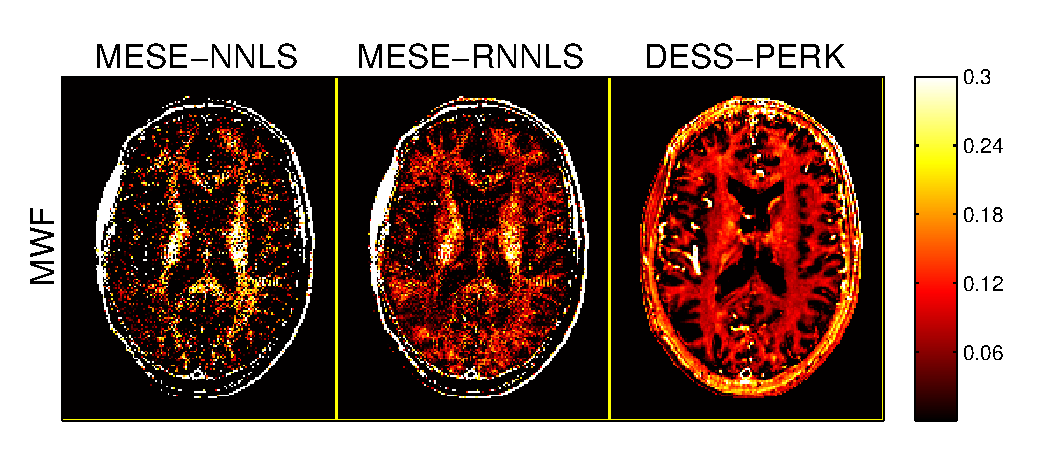
\includegraphics [width=\textwidth] {brain/mese-mw,dess-ff,sl-5.eps}
	\caption{%
		Representative NNLS and RNNLS $\mwf$ estimates 
		from a MESE acquisition 
		alongside a PERK $\ff$ estimate 
		from a precision-optimized DESS acquisition,
		in the brain of a healthy volunteer.
		Using similar signal reception imaging parameters,
		MESE $\mwf$ estimates 
		required $40$m$6$s total scan time
		while DESS $\ff$ estimates
		required $7$m$45$s total scan time. 
		PERK $\ff$ estimates exhibit less WM variation
		and more clearly delineate cortical WM/GM boundaries
		than MESE $\mwf$ estimates.
		Table~\ref{tab:mwf,invivo} 
		presents corresponding sample statistics
		computed over manually selected WM and GM ROIs.
	}%
	\label{fig:mwf,invivo}
\end{figure}

% mese-rnnls and dess-perk lateral wm values appear visually similar
% rnnls values appear lower but show less variation than nnls maps, due to regularization
% mese estimates higher in medial regions
% 	similar spatial pattern to simulations, perhaps due to b1 errors
% 	lower values in internal capsules may be due to overlap between mw and iew peaks zhang:15:com
Fig.~\ref{fig:mwf,invivo} compares 
NNLS and RNNLS $\mwf$ estimates from MESE scans
as well as PERK $\ff$ estimates from optimized DESS scans.
PERK $\ff$ estimates exhibit less WM variation
and more clearly delineate cortical WM/GM boundaries
than MESE $\mwf$ estimates.
RNNLS $\mwf$ estimates are visibly lower than NNLS $\mwf$ estimates
due to regularization
but exhibit reduced WM variation,
somewhat improving visualization of WM tracts. 
RNNLS $\mwf$ and PERK $\ff$ estimates 
appear visually similar in lateral WM regions,
but both NNLS and RNNLS $\mwf$ estimates are elevated in medial regions.
MESE $\mwfest$ overestimation in internal capsules (IC)
has been attributed 
to overlap in NNLS $\Tt$ spectrum estimates 
of the myelin water and cellular water $\Tt$ peaks \cite{zhang:15:com}.
We additionally observe
that MESE $\mwf$ estimates exhibit similar spatial variation
here versus in simulations 
(\cf Figs.~\ref{fig:mwf,2comp}-\ref{fig:mwf,3comp})
suggesting that some WM spatial variation
in MESE $\mwf$ estimates
may be attributable to flip angle variation,
despite compensation for transmit field inhomogeneity.

\begin{table}[!t]
	\centering
	\small
	\begin{minipage}{0.19\textwidth}
		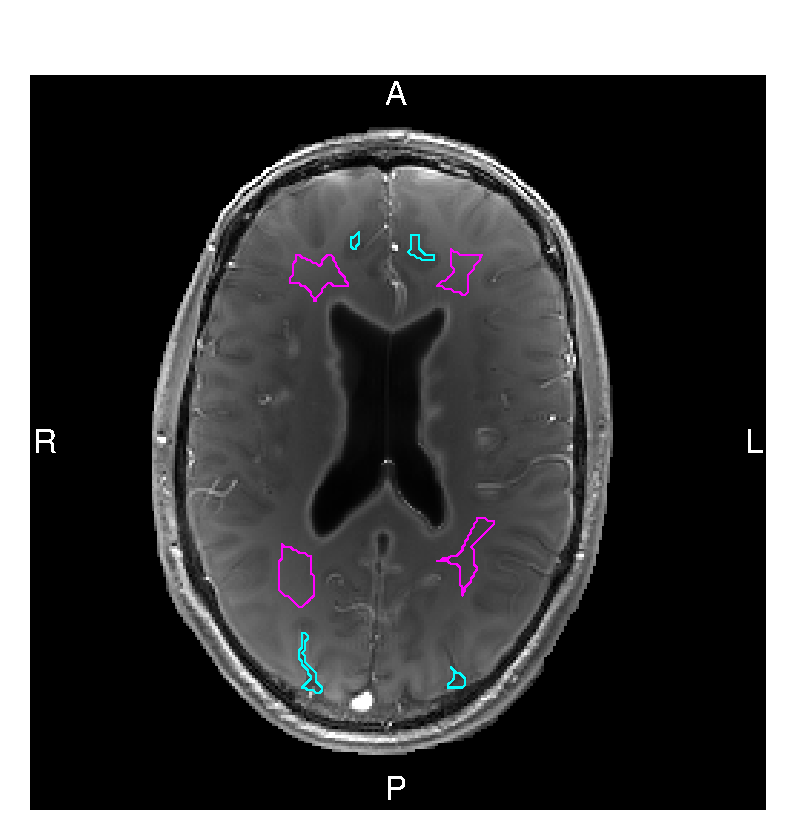
\includegraphics [width=\textwidth] {brain/roi.eps}
	\end{minipage}
	\begin{minipage}{0.78\textwidth}
		\begin{tabu} {c | r r r}
			\hline
			\hline
			ROI 		& MESE-NNLS $\mwfest$ 	& MESE-RNNLS $\mwfest$	& DESS-PERK $\ffest$ 	\\
			\hline
			\RA WM 	& \mnstd{0.09}{0.096}   & \mnstd{0.074}{0.055} 	& \mnstd{0.117}{0.019}	\\
   		\LA WM 	& \mnstd{0.066}{0.086}  & \mnstd{0.054}{0.041}  &	\mnstd{0.100}{0.0119}	\\
   		\RP WM 	& \mnstd{0.047}{0.074}  & \mnstd{0.044}{0.041} 	&	\mnstd{0.093}{0.019}	\\
   		\LP WM 	& \mnstd{0.116}{0.098}  & \mnstd{0.075}{0.050}  &	\mnstd{0.0870}{0.0114}\\
  		\IC WM 	& \mnstd{0.211}{0.133}  & \mnstd{0.178}{0.083}  &	\mnstd{0.111}{0.0241}	\\
 			\AC GM 	& \mnstd{0.007}{0.024}  & \mnstd{0.010}{0.017} 	&	\mnstd{0.019}{0.045}	\\
			\hline
			\hline
		\end{tabu}
	\end{minipage}
	\caption{%
		\emph{Left}:
		WM/GM ROIs,
		overlaid on a representative anatomical
		MESE first-echo image.
		Separate lateral WM ROIs are distinguished
		by anterior-right (\RA),
		anterior-left (\LA),
		posterior-right (\RP),
		and posterior-left (\LP) directions
		and are respectively comprised
		of $90$, $79$, $182$, and $201$ voxels.
		Two internal capsule (\IC) polygons
		are pooled into a single medial WM ROI
		comprised of $347$ voxels.
		Three small anterior cortical (\AC) GM polygons
		are pooled into a single GM ROI
		comprised of $78$ voxels.
		\emph{Right}:
		Sample means $\pm$ sample standard deviations
		of NNLS/RNNLS $\mwf$ estimates 
		from a MESE acquisition
		as well as PERK $\ff$ estimates 
		from an optimized DESS acquisition,
		computed over WM/GM ROIs.
		Each sample statistic is rounded off
		to the highest place value
		of its (unreported) standard error,
		computed via formulas in \cite{ahn:03:seo}.
		Fig.~\ref{fig:mwf,invivo} presents corresponding images.
	}%
	\label{tab:mwf,invivo}
\end{table}

% dess-perk has lower within-roi variation in wm (higher in gm)
% dess-perk has more similar estimates across wm rois
% rnnls has lower estimates, less wm variation than nnls (said above)
% nnls and rnnls sig higher in ic wm than in lateral wm rois
% dess perk significantly different estimates than mese fm in several wm rois, though comparable to other studies (see alonso-ortiz) for a review)
% no methods measure significant myelin water content in ac gm
Table~\ref{tab:mwf,invivo} summarizes sample statistics
of NNLS/RNNLS $\mwf$ estimates from MESE scans
and PERK $\ff$ estimates from optimized DESS scans,
separately computed over four lateral WM ROIs
containing $90$, $79$, $182$, and $201$ voxels;
one pooled medial IC WM ROI containing $347$ voxels;
and one pooled anterior cortical (AC) GM ROI containing $78$ voxels.
PERK $\ff$ estimates exhibit the lowest variation within WM ROIs
and the most similar sample means across WM ROIs.
NNLS and RNNLS $\mwf$ sample means are significantly higher 
in the IC WM ROI than in lateral WM ROIs,
possibly due to overlap in NNLS $\Tt$ spectrum peaks
and/or to flip angle spatial variation
(as described in the previous paragraph).
PERK $\ff$ sample means differ significantly 
from RNNLS $\mwf$ sample means
in several WM ROIs,
though PERK WM $\ff$ sample means are consistently comparable
with literature MESE measurements
(\eg, see \cite{alonsoortiz:15:mbm} for a review).
Neither the NNLS/RNNLS $\mwfest$ nor PERK $\ffest$ estimators
measured significant myelin water content in AC GM.

%%%%%%%%%%%%%%%%%%%%%%%%%%%%%%%%%%%%%%%%%%%%%%%%%%%
\section{Discussion}
\label{s,mwf,disc}
%%%%%%%%%%%%%%%%%%%%%%%%%%%%%%%%%%%%%%%%%%%%%%%%%%%

% first work to demonstrate wm myelin imaging from ss scans similar to mese mwf estimates
% mese-rnnls mwf and dess-perk estimates may be comparable in some regions of lateral wm
% higher-snr mese-rnnls studies (perhaps ex vivo) required to ascertain strength of similarity
% nevertheless, this feasibility study demonstrates myelin content quantification 
Simulations and experiments demonstrate the feasibility
of myelin water content quantification
from a fast precision-optimized DESS MR acquisition.
It remains challenging to assess
whether DESS $\ff$ estimates are comparable
to MESE $\mwf$ estimates \invivo
because of high MESE $\mwf$ estimation variation.
For greater confidence in comparisons,
future \exvivo studies in excised brain tissue
would allow for longer MESE scans
without increasing motion-induced errors
and would thereby enable 
more precise MESE $\mwf$ estimation.
Studies at higher field strengths
would also enable more precise estimation
due to higher SNR.
Nevertheless,
the experiments described herein
are the first to demonstrate
\invivo lateral WM myelin water content estimates
from a fast SS MR acquisition
that are at all similar 
to conventional MWF estimates
from a slower MESE MR acquisition.

% experiments also provide evidence that perk scales well while maintaining accuracy
% in 2d simulations with unrealistically narrow grid searches, 
% 	perk consistently at least 500x faster including training time 
% 	and in both simulations achieves lower rmses
% omitted ml estimation in vivo because ml estimates suffered strong wm overestimation 
%		in 3-compartment simulation with modest model mismatch 
%		(despite grid search constraints that distinguish compartments to reduce chance of errors due to multiple global minima)
% more realistic grid searches on other optimized in vivo datasets took 68 cpu days and were still unable to reliably distinguish compartments due possibly to multiple global minima
% taking results together, we have evidence that perk scales considerably better than grid search and may be more appropriate than grid search for challenging problems with multiple minima.
Taken together with the results presented
in Ch.~\ref{c,perk},
experiments herein also provide evidence
that the PERK estimator \cite{nataraj:17:dfm-arxiv}
can maintain reasonable accuracy
while scaling gracefully
with the number of latent parameters per voxel. 
In simulations,
PERK consistently took at least $500\times$ less time
and consistently achieved lower WM RMSE
than an ML estimator 
achieved via unrealistically narrow grid search
around the ground truth.
In preliminary experiments
on other precision-optimized \invivo datasets
from the same healthy volunteer,
PERK took comparable time 
and produced similar $\ff$ estimates 
as reported here
while a more realistically constrained grid search
took about $68$ CPU-days 
running on $24$ nodes of a computing cluster
and did not produce reasonable $\ff$ estimates.
To avoid the confounding possibility of \invivo ML errors
due to multiple global minima,
we included narrowly constrained grid search estimates
from a 3-compartment simulation here
and from poor ML accuracy conclude
that the ML estimator is more sensitive 
to model mismatch than the PERK estimator
for this application.
These results suggest 
that PERK scales much better than grid search
with the number of latent parameters per voxel
and that PERK may be more more robust than grid search
to multi-compartmental modeling errors.

% both here and in other runs, optimized profiles consist of mostly dess scans
% since for fixed te and no exchange, spgr only provides multicompartment t1 contrast,
%		this suggests that multi-compartment t2 sensitivity mostly arises from dess
% both here and in other runs, optimized scan profile has tr diversity, even at the expense of fewer scan than possible under time budget
% in unreported studies, tried optimizing with implicit min tr restrictions; saw substantial degradation in optimized ff precision
% suggests dess tr (in add. to flip) variation important for ff estimation
Despite freedom to design arbitrary combinations
of SPGR and DESS scans,
the optimized acquisition used here
as well as several other unreported acquisitions 
designed under different total time constraints
consisted either entirely or mostly of DESS scans.
Since the two-compartment SPGR signal models 
used in acquisition design
depend on $\tf{1},\ts{1}$ but not $\tf{2},\ts{2}$,
DESS-dominated scan designs suggest 
that multi-compartmental $\Tt$ effects
give rise to $\ff$ sensitivity in SS sequences
more so than multi-compartmental $\To$ effects.
Somewhat surprisingly,
reported and unreported precision-optimized acquisitions 
also exhibit substantial $\TR$ variation across scans,
even at the expense
of fewer scans than possible 
under time constraints.
In further unreported studies,
we investigated this phenomenon 
by repeating scan optimization
while implicitly constraining repetition times to be minimal.
We consistently observed substantial ($\sim$10-20\%) degradation
in expected $\ff$ relative standard deviation,
suggesting that $\TR$ variation 
(in addition to flip angle variation)
is important for designing acquisitions
that enable precise $\ff$ estimation.

% mese mwf and dess ff use different model assumptions, objective functions, and algorithms that may limit their comparability even with high snr
% omit: mese mwf allows for arbitrary numbers of compartments but assumes bulk t1 known
% omit: dess ff allows for compartmental t1 variation but fixes to two compartments
% omit: both neglect exchange, compartmental off-resonance effects
% for more similar model assumptions, could attempt to optimize dess for estimating three or more compartments (or use mese to estimate fewer compartments)
% with bulk t1,kappa assumption, both mese and dess could be solved with (r)nnls objectives
% perhaps without bulk t1, kap could solve both mese and dess with perk
% in general, estimating more parameters constitutes more challenging problems that will likely require more (MESE or DESS) data
Even with high SNR,
differences in model assumptions, objective functions, and estimation algorithms
may limit the quantitative comparability 
of DESS $\ff$ imaging as implemented here
and MESE $\mwf$ imaging as implemented here and in original works 
\cite{mackay:94:ivv,whittall:89:qio}.
For more similar model assumptions,
one could attempt to estimate 
from a suitably optimized DESS acquisition
a $\Tt$ (or joint $\paren{\To,\Tt}$) distribution
using two-, three-, or higher-compartment models
and correspondingly estimate from MESE data
a more coarsely sampled 
$\Tt$ (or joint $\paren{\To,\Tt}$) distribution.
If $\stx,\To$ maps are known
and non-exchanging additive models are employed,
one could estimate $\Tt$ distributions
from both MESE and DESS data 
using NNLS or RNNLS objective functions.
With weaker model assumptions 
that cause signal models to be nonlinear in unknowns,
one could estimate distributions using PERK.
This work focused on demonstrating the feasibility
of myelin water quantification
using a simple two-compartment model 
of a fast DESS acquisition;
estimating more unknowns 
from more complicated (MESE or DESS) models
will at least necessitate more scans
and may still prove challenging.

% omit: b1 sensitivity

%%%%%%%%%%%%%%%%%%%%%%%%%%%%%%%%%%%%%%%%%%%%%%%%%%%
\section{Conclusion}
\label{s,mwf,conc}
%%%%%%%%%%%%%%%%%%%%%%%%%%%%%%%%%%%%%%%%%%%%%%%%%%%

This chapter has introduced 
a fast SS MRI acquisition
for precise myelin water imaging.
The acquisition consists
of three DESS scans
whose flip angles and repetition times
have been optimized 
under an aggressive time constraint
to enable precise estimation
of the faster-relaxing signal fraction $\ff$ 
in a simple two-compartment DESS model.
Simulations without model mismatch demonstrate
that PERK and ML $\ff$ estimates
from the proposed DESS acquisition
exhibit comparable RMSEs,
but PERK is more than $500\times$ faster.
Simulations with modest levels of model mismatch demonstrate
that conventional MESE $\mwf$ estimates are sensitive 
to unaccounted variable $\To$-recovery rates across compartments
and accounted flip angle spatial variation
while DESS $\ff$ estimates are sensitive 
to relaxation in an unaccounted third compartment,
suggesting limited quantitative comparability 
of MESE $\mwf$ and DESS $\ff$ WM estimates. 
\Invivo experiments are nevertheless the first to demonstrate
lateral WM myelin water content estimates
from a fast SS acquisition
that are similar 
to conventional MWF estimates
from a slower MESE MR acquisition.

% need to first build support for claim that ff as measured by spgr/dess 
% is a measure of mwf as measured originally by mackay
% need to compare our estimates with estimates from a mese measurement
% foreseen challenges: still will be differences in model assumptions and estimation algorithms
\paragraph{Comparisons with MESE MWF Estimates}
We would like to claim
that fast-relaxing fraction $\ff$ estimates
from precision-optimized SPGR/DESS scan profiles
are accurate measurements 
of MWF as originally defined 
in \cite{mackay:94:ivv}.
To build support
for this hypothesis,
we will need
to systematically compare our $\ff$ estimates
with MWF estimates
from a MESE acquisition.
Such comparison is challenging
because the methods differ
not only in acquisitions
but also in modeling assumptions
\footnote{MESE MWF estimation 
	assumes $\To$ is known and fixed
	over many compartments.
	As presented, SPGR/DESS $\ff$ estimation
	assumes unknown variable $\To$
	across two compartments.
	Both models neglect exchange 
	and multi-compartmental off-resonance effects,
	and assume known flip angle spatial variation.
	\label{foot:mwf,assumption}
},
initialization
(KRR estimate \eqref{eq:krr,x-hat}
versus the zero vector),
objective functions
(ML cost \eqref{eq:relax,lf-mtx}
versus a regularized nonnegative least-squares (NNLS) cost
\cite[Eq.~8]{whittall:89:qio}),
and estimation algorithms
(gradient projection method \cite{rosen:60:tgp}
versus
least-distance programming (LDP) \cite[\S23.4]{lawson:74}).

% first validate krr by comparing mwf estimates from nnls/ldp vs krr, using same model
% then take as many assumptions same as possible while comparing mese and spgr/dess
% modify model (possibly of both acq) as needed to achieve agreement
We plan to approach validation as follows.
First,
we will compare \invivo MWF estimates
from a fixed signal model
of a fixed MESE acquisition
using KRR, KRR-initialized ML,
KRR-initialized regularized NNLS,
and zero-initialized regularized NNLS
\footnote{Both KRR- and zero-initialized NNLS 
	should yield near-equivalent solutions
	because the regularized NNLS problem is convex,
	assuming as in \cite{whittall:89:qio, mackay:94:ivv}
	that all latent parameters other than MWF are known.
}.
Here, 
all three iterative algorithms can be solved
via gradient projection method
for consistency.
These results will provide direct insight
as to how KRR and KRR-initialized ML estimation perform
for \invivo MWF estimation
from a classical acquisition and signal model.
% mese takes t1 as known as and constant across compartments from IR-prepared FSE sequences
% we estimate t1 for two compartments
% joint estimation of refocusing flip angle; we assume flip angle scaling known

% little bit of a trivial problem above (linear)
% next study nonlinear but relatively simple problem mwf and flip estimation
% t1 still known
% can't use nnls but can use krr and varpro 
% classical acquisition but more complicated signal model
Using KRR as above
for a convex MWF estimation problem 
is important for systematic validation
but is overkill in practice.
For a more interesting usage,
we will next consider joint estimation
of MWF and transmit field variation $\stx$
(still assuming knowledge of other latent parameters)
from the same MESE dataset.
NNLS is inapplicable 
for this non-convex problem;
however, 
we can still quickly validate KRR estimates 
via voxel-wise exhaustive grid search
due to low problem dimensionality.
If promising,
these results will support the claim
that KRR could be useful 
for fast \invivo MWF estimation 
from nonlinear models.

% next, could fix model assumptions 
% design spgr/dess acquisition for estimating ff from much simpler model
% this model will again lead to convex problem in ff that can be solved via above methods
% positive result here suggests that spgr/dess can be used to design mwf acquisitions
To compare SPGR/DESS and MESE acquisitions,
we can modify SPGR/DESS model assumptions
to those taken in \cite{prasloski:12:rwc}
for the MESE model
(listed in Footnote~\ref{foot:mwf,assumption})
and thereby formulate an analogous
$\Tt$ distribution estimation problem,
for which linear algorithms 
such as regularized NNLS and LDP are applicable.
Our task will then be 
to design a fast SPGR/DESS acquisition
under these modified model assumptions
that permits precise voxel-wise estimation 
of the $\Tt$ distribution.
The resulting estimated $\Tt$ distributions
will be directly comparable 
to $\Tt$ distributions 
from MESE acquisitions
and could be used
to form SPGR/DESS MWF maps
that are directly comparable 
with MESE MWF maps.

% finally, show true generality of methods developed in thesis
% can relax some model assumptions, design corresponding scans, and study via krr/ml only
% e.g., variable t1 over two discrete compartments gives acquisition in table mwf,acq
% others might be three discrete compartments or exchange (though this is hard w/ acq design)
% comparing with KRR-ML spgr/dess gives info about effect of model assumptions
Upon isolated validation
of acquisitions, initializations, and estimation algorithms,
we can explore the effects 
of different modeling assumptions
using the full flexibility
of optimized scan design and KRR estimation.
As a first experiment,
we could try to optimize
under the variable-$\To$ two-compartment model 
a MESE acquisition
similar to the SPGR/DESS acquisition 
presented in Table~\ref{tab:mwf,acq}
and compare resulting SPGR/DESS and MESE $\ffest$ maps. 
If $\ffest$ from these models do not measure MWF
with sufficient specificity,
we could explore similar comparisons
using more complicated models
involving exchange, three (or more) compartments,
and/or compartmental off-resonance effects.
All of these model comparisons 
will require highly nonlinear estimation problems
involving many latent parameters,
for which KRR-initialized ML estimation is well-suited.

% comparison with mt
% different measure of myelination - does it correlate?
\paragraph{Comparisons with Different Myelin Biomarkers}
We are also interested
in how $\ff$ estimates (or other MWF proxies)
correlate with other myelin biomarkers. 
One contending noninvasive marker arises
from MR pulse sequences sensitized
to the inhomogeneous magnetization transfer (ihMT) effect
\cite{varma:15:mtf},
which has recently been argued
to be specific
to the large membrane lipids
that comprise much of myelin
\cite{varma:15:iom, swanson:17:mda}.
Outside MRI,
invasive measurements
from histology
have been used to study myelin 
(as in \eg, \cite{gareau:00:mta, webb:03:imt})
and could serve as a gold-standard \insitu marker.
Multi-compartmental and ihHT MRI markers 
can be successively compared 
through phantom, healthy volunteer, and patient studies.
Both MRI and histological markers
can be compared through 
phantom and \insitu studies.
All of these studies
are highly amenable 
to clinical collaborations.
